\documentclass{article}

% if you need to pass options to natbib, use, e.g.:
\PassOptionsToPackage{numbers, sort&compress}{natbib}
% before loading neurips_2026

% The authors should use one of these tracks.
% Before accepting by the NeurIPS conference, select one of the options below.
% 0. "default" for submission
\usepackage[main,final]{neurips_2026}
% the "default" option is equal to the "main" option, which is used for the Main Track with double-blind reviewing.
% 1. "main" option is used for the Main Track
%  \usepackage[main]{neurips_2026}
% 2. "position" option is used for the Position Paper Track
%  \usepackage[position]{neurips_2026}
% 3. "eandd" option is used for the Evaluations & Datasets Track
 % \usepackage[eandd]{neurips_2026}
% 4. "creativeai" option is used for the Creative AI Track
%  \usepackage[creativeai]{neurips_2026}
% 5. "sglblindworkshop" option is used for the Workshop with single-blind reviewing
 % \usepackage[sglblindworkshop]{neurips_2026}
% 6. "dblblindworkshop" option is used for the Workshop with double-blind reviewing
 % \usepackage[dblblindworkshop]{neurips_2026}
% 7. "education" option is used for the Education Track
 % \usepackage[education]{neurips_2026}


% After being accepted, the authors should add "final" behind the track to compile a camera-ready version.
% 1. Main Track
 % \usepackage[main, final]{neurips_2026}
% 2. Position Paper Track
% \usepackage[position, final]{neurips_2026}
% 3. Evaluations & Datasets Track
 % \usepackage[eandd, final]{neurips_2026}
% 4. Creative AI Track
% \usepackage[creativeai, final]{neurips_2026}
% 5. Workshop with single-blind reviewing
% \usepackage[sglblindworkshop, final]{neurips_2026}
% 6. Workshop with double-blind reviewing
% \usepackage[dblblindworkshop, final]{neurips_2026}
% Note. For the workshop paper template, both \title{} and \workshoptitle{} are required, with the former indicating the paper title shown in the title and the latter indicating the workshop title displayed in the footnote.
% For workshops (5., 6.), the authors should add the name of the workshop, "\workshoptitle" command is used to set the workshop title.
% \workshoptitle{WORKSHOP TITLE}
% 7. Education Track
% \usepackage[education, final]{neurips_2026}

% "preprint" option is used for arXiv or other preprint submissions
 % \usepackage[preprint]{neurips_2026}

% to avoid loading the natbib package, add option nonatbib:
%    \usepackage[nonatbib]{neurips_2026}

\usepackage[utf8]{inputenc} % allow utf-8 input
\usepackage[T1]{fontenc}    % use 8-bit T1 fonts
\usepackage{hyperref}       % hyperlinks
\usepackage{placeins}
\usepackage{graphicx}       % figures
\usepackage{float}          % [H] tables stay with their text
\usepackage{url}            % simple URL typesetting
\usepackage{booktabs}       % professional-quality tables
\usepackage{amsfonts}       % blackboard math symbols
\usepackage{amsmath}        % math environments
\usepackage{amssymb}        % math symbols
\usepackage{nicefrac}       % compact symbols for 1/2, etc.
\usepackage{microtype}      % microtypography
\usepackage{xcolor}         % colors
\usepackage{textcomp}       % cent sign in the reward table
\setlength{\textfloatsep}{11pt}
\setlength{\intextsep}{9pt}
\setlength{\floatsep}{11pt}

% Section numbers carry a trailing dot in the heading (cross-references unchanged).
\makeatletter
\renewcommand{\@seccntformat}[1]{\csname the#1\endcsname.\quad}
\makeatother

% Note. For the workshop paper template, both \title{} and \workshoptitle{} are required, with the former indicating the paper title shown in the title and the latter indicating the workshop title displayed in the footnote.
\title{One Shared Bounded-Beta PPO Policy for Zero-Shot Commercial HVAC Control}


% The \author macro works with any number of authors. There are two commands
% used to separate the names and addresses of multiple authors: \And and \AND.
%
% Using \And between authors leaves it to LaTeX to determine where to break the
% lines. Using \AND forces a line break at that point. So, if LaTeX puts 3 of 4
% authors names on the first line, and the last on the second line, try using
% \AND instead of \And before the third author name.


\author{%
  Sidharthan S \\
  Independent Researcher \\
  \texttt{sid250581@gmail.com} \\
  % examples of more authors
  % \And
  % Coauthor \\
  % Affiliation \\
  % Address \\
  % \texttt{email} \\
  % \AND
  % Coauthor \\
  % Affiliation \\
  % Address \\
  % \texttt{email} \\
  % \And
  % Coauthor \\
  % Affiliation \\
  % Address \\
  % \texttt{email} \\
  % \And
  % Coauthor \\
  % Affiliation \\
  % Address \\
  % \texttt{email} \\
}


\raggedbottom

\begin{document}
\nocite{goldfeder2024smart,goldfeder2026smart}


\maketitle
\thispagestyle{empty}  % no page number on the title page


\begin{abstract}
Heating, ventilation, and air-conditioning (HVAC) systems govern indoor environmental quality in modern buildings under the dual imperative of cutting energy and carbon while preserving comfort. This remains difficult because building dynamics, weather, and occupancy vary, so controllers are tuned per building. We show that a single shared Proximal Policy Optimization (PPO) policy, trained solely on the benchmark's 3C (comfort, cost, and carbon) reward, transfers zero-shot across heterogeneous buildings. Trained on 30 scenarios across six layouts and five climates, it scores 0.0165 versus 0.0461 for the shipped PID controller over 90 held-out months and 0.0098 versus 0.0437 over 54 more, the lowest mean on both sets, below the controller on 143 of 144 months, holding on two unseen buildings and one climate. For a Soft Actor-Critic (SAC) baseline, the action representation, not the learning algorithm, blocks transfer: holding scenarios, fixed-width input, seed, and 50M budget fixed, replacing a Gaussian policy with a bounded Beta distribution improves SAC from 0.0457 to 0.0338 on 90 held-out months and from 0.0644 to 0.0261 on one unseen building, improving every building. PPO with the same Beta distribution adds the rest, reaching 0.0165 at full budget and outperforming the PID controller on all five buildings, whereas SAC still loses on the other unseen building. A fixed-width layout, bounded Beta distribution, and PPO let one policy span 30 to 85 zones without per-building training. More broadly, aligning action bounds with physical actuators unlocks zero-shot infrastructure control, though findings remain inside simulation.
\end{abstract}


\section{Introduction}

\textbf{Context}: Achieving global decarbonization depends heavily on reducing the environmental footprint of the built environment. According to the United Nations Environment Programme \citep{unep2025buildings} and the International Energy Agency \citep{iea2018futureofcooling}, the buildings and construction sector accounts for 34\% of global energy and process $\text{CO}_2$ emissions. Rather than declining in line with climate targets, sector-wide operational emissions rose from 9.3 $\text{GtCO}_2$ in 2015 to a record 9.8 $\text{GtCO}_2$ in 2023, representing a 5.4\% increase. Commercial (non-residential) buildings alone contribute 10\% of total global emissions \citep{eia2018cbecs}, which constitutes roughly 29.4\% of all building-sector emissions. The operational footprint of these facilities is driven primarily by heating, ventilation, and air-conditioning (HVAC) systems.

\textbf{Building control:} A building's HVAC infrastructure consists of interconnected thermal zones served by a central network of heating, cooling, and air-distribution equipment. A central plant supplies heated and chilled water to air-handling units (AHUs), which condition and distribute air through duct networks, while variable air volume (VAV) boxes regulate the airflow delivered to individual zones through dampers and local reheat coils. A building controller monitors measurements from the zones and central plant and acts at both levels: it sets the plant and air-handler operating points, such as hot-water loop temperature and supply-air temperature, and it positions the zone dampers and reheat valves. Rather than directly setting individual zone temperatures, these commands influence the thermal environment indirectly through the building's HVAC equipment and physical dynamics.

\textbf{Challenges in Smart Building Control:} Controlling HVAC systems in commercial buildings presents several interconnected challenges. \textbf{First}, buildings exhibit substantial thermal inertia: structural mass, floors, and furnishings absorb and release heat gradually. \textbf{Second}, occupancy decides where the objective is charged. As occupants arrive and depart, thermal and ventilation demand shifts across zones, and the score bills comfort only in occupied zones while it bills energy and carbon at every step. A controller has to let the empty zones drift, and it sees only a building-wide occupant count. \textbf{Third}, the same building needs different supply-water and supply-air temperatures in a cold month and a warm one, so a controller that covers both has to move its operating point with the weather rather than hold one setting. To investigate these challenges, the \textbf{Smart Buildings Control Suite} \citep{goldfeder2024smart} provides a standardized environment comprising measured building data, building-specific calibrated simulation environments, and a common control interface.

\textbf{Key contribution:} One PPO recipe, trained once, transfers to buildings it has never seen.
\begin{itemize}
\item \textbf{Zero-shot multi-building transfer.} One 453K-parameter PPO \citep{schulman2017proximal} policy with no per-building tuning, dynamics model, or residual controller scores 0.0165 on 90 held-out months and 0.0098 on 54 more against 0.0461 and 0.0437 for the shipped controller, the lowest mean of the five on both sets and below the controller on 143 of 144 months, with two unseen buildings (of eight) and one unseen station (of six).
\item \textbf{The action representation, not the learning algorithm.} The bounded Beta head represents each actuator over its full range, with a shape that can be a hump or a U, so a damper can be held open or shut; a standard Gaussian cannot. Holding the scenarios, the fixed-width input, the seed and the 50M budget fixed, replacing that Gaussian with the Beta head improves a Soft Actor-Critic (SAC) \citep{haarnoja2018sac} baseline from 0.0457 to 0.0338 on the 90 months and from 0.0644 to 0.0261 on one unseen building; every building improves. PPO with the same Beta head adds the rest, reaching 0.0165 at its full budget and staying below the controller on all five buildings, while SAC still loses on the other unseen building (Appendix~I).
\item \textbf{A measured recipe on an open stack.} Staggered starts, per-head ratio clipping, and a cap on Beta certainty carry the result (2.213, 0.152, and 0.054 without them, against 0.033 at 50M steps), running on a modified PufferLib trainer and a CUDA port at 6,200 steps/s on one RTX 3090 (42$\times$ the reference simulator on 12 CPU cores).\footnote{Code: \url{https://github.com/Sidharth1743/NeurIPS2026_Smart_Building_Challenge}}
\end{itemize}
\section{Related Work}

\textbf{Benchmark:} Reinforcement learning has been applied to HVAC control from individual thermal zones to whole-building energy management \citep{wei2017deep,yu2021review}, and a notable real deployment reports 9\% and 13\% energy savings across two commercial facilities \citep{luo2022controlling}. Interacting with buildings is costly, and model-predictive control needs a calibrated model of every building \citep{afram2014theory}, so the Smart Buildings Control Suite trains agents in calibrated simulators built from real telemetry \citep{blum2019prototyping,goldfeder2024smart}. The Smart Buildings Challenge then adds procedurally generated buildings and held-out configurations, to ask whether a learned controller transfers across unseen buildings and climates \citep{goldfeder2026smart}.

\textbf{Offline and online reinforcement learning:} HVAC control studies differ in how agents acquire their experience. Offline reinforcement learning learns from previously collected logs, which avoids exploration and cannot test alternatives the logs never contain \citep{blad2022data,levine2020offline}. Simulation-based training provides a safer setting for exploring alternative control strategies, while recent studies have also investigated transferring simulation-trained policies to real buildings through online adaptation \citep{coraci2023online}. We instead train interactively in simulation, so the policy learns from newly generated experience rather than fixed logs.

\textbf{Scalability and generalization across buildings:} Transfer learning reuses a controller trained on source buildings: cross-building transfer of pretrained DQN controllers \citep{fang2023cross}, multi-source transfer for multi-zone control \citep{hou2024multi}, heterogeneous transfer across buildings with different energy systems and state representations \citep{coraci2024heterogeneous}. Each adapts a pretrained controller to a target building; we instead train one shared policy across heterogeneous buildings at once, without target-specific fine-tuning.

\section{Methods}

\subsection{Problem Formulation and Control Environment}

We formulate building climate control as a discrete-time \textbf{partially observed Markov decision process (POMDP)}, $(\mathcal{S}, \mathcal{A}, \mathcal{T}, \mathcal{R}, \Omega, \mathcal{O}, \gamma)$ \citep{garcia2013mdp,sutton2018reinforcement}. Table~\ref{tab:interface} gives the observation, the hybrid action space and the reward.

\begin{table}[h]
\centering
\small
\renewcommand{\arraystretch}{1.35}
\begin{tabular}{@{}p{0.21\linewidth}p{0.73\linewidth}@{}}
\toprule
space / representation & Parameters and ranges \\
\midrule
\textbf{Observation ($o_t$)} & Flat float32 vector of building-dependent length ($d$): zone temperatures, heating/cooling setpoints, flows, damper and reheat echoes, AHU supply/static states, loop temperatures and pressures; 16 of the 48 supplied diurnal and weekly harmonics; two comfort flags; building-wide occupancy, $(n-125)/126$. \\
\addlinespace[3pt]
\textbf{Action ($a_t$)} & $a^{\text{cont}}\in[-1,1]^{3K+2V+2}$, $a^{\text{disc}}\in\{0,1\}^{K+1}$. Supply air 285--305 K; supply water 310--350 K; static pressure 0--2000 Pa; loop differential pressure 0--20; damper, reheat and recirculation $[0,1]$; on/off for the $K$ handlers and the pump. \\
\addlinespace[3pt]
\textbf{Reward ($r_t$)} & Comfort $C_1$ (occupancy-weighted productivity, \$300 per occupant-hour), energy cost $C_2$ (hourly electricity price of 16--20\,\textcent/kWh plus a monthly gas price) and carbon emission $C_3$ (hourly grid intensity of 87.8--104.7\,g/kWh plus a constant gas rate of 0.1813\,kg/kWh); all non-positive, unclipped, and zero at the ideal. \\
\addlinespace[3pt]
\textbf{Horizon} & $\Delta t=300$ s; $T=8{,}640$ steps (30 days); discounted training return with $(\gamma,\lambda)=(0.99,0.95)$; evaluation is the negated undiscounted mean per-step reward, averaged across scenarios. \\
\bottomrule
\end{tabular}
\vspace{4pt}
\caption{The control interface of the benchmark environment.}
\label{tab:interface}
\end{table}

The dynamics are \textbf{deterministic} given the commands and the scenario's weather trace: thermal mass delays the response by minutes to hours. Randomness enters only through occupancy. The controller never sees the full state: the mass temperature inside each control volume, the occupancy of an individual zone (only a building-wide count is reported), and the building's identity, weather name or month (only diurnal and weekly harmonics are given). The policy recovers the missing per-zone and temporal context from history (\S3.3); Appendix~A gives the model and Appendix~B the input contract.

The policy acts \textbf{directly on the equipment}, without a rule-based sequence or safety filters. Whatever behavior it shows is learned from interaction with the simulator.

{\samepage
Each step returns the benchmark's \textbf{3C reward} in the benchmark's notation,
\[
r_t = 0.6\,C_1 + 0.2\,C_2 + 0.2\,C_3,
\]
where $C_1 \le 0$ is the occupancy-weighted comfort term, scored against the standard thermal-comfort band of the benchmark \citep{ashrae55} (zero inside the band and whenever the building is empty, falling linearly over the first 5 K outside it and quadratically beyond), $C_2 \le 0$ the energy cost and $C_3 \le 0$ the carbon emission. No term is clipped, and the objective is unmodified: no shaping, potential or extra comfort term.
}

% NOTE (content.md, not paper prose): What to move to the appendix so this stays a subsection: the arity formula in words, field ordering and the `_1` collision convention, missing-value fill, the full state enumeration, the exact normalization denominators, the per-op float32 decode identity, and the two-level score definition with its equation. None of them are needed to follow \S3.2--\S3.5, and all are needed by someone re-implementing you.
% NOTE (content.md, not paper prose): One judgment call worth making deliberately: keep the ``no building identifier'' clause in \S3.1 rather than in \S3.5. It reads there as a property of the interface, not as a defense of a claim, and it is the sentence that makes your generalization result about the policy instead of about the data.

\subsection{GPU-Accelerated Simulation Infrastructure}

To enable large-scale parallel training, we port the complete building simulation environment to CUDA, integrating the environment with PufferLib's vector interface \citep{suarez2024pufferlib} and CUDA graph execution. With double-precision physics, the implementation sustains 12K environment steps per second (SPS) on an NVIDIA L40S. Implementation details, validation and throughput are in Appendix~A.

\subsection{Shared Policy Architecture and Observation Design}

One policy must control buildings of different size with a single set of weights. We achieve that with two choices: an interface identical for every building, and readouts shared by equipment role rather than by zone.

Buildings differ in their numbers of zones and air handlers, so their raw observations are structurally incompatible. We map every building into the same 983-value vector: 90 zone slots, 9 air-handler slots, one hot-water slot and one global slot. Absent slots are zero, device fields are returned to physical units with the constants the gateway supplies, and each group is put on a fixed scale, so the same slot means the same thing in every building (Figure~\ref{fig:arch}; Appendix~B).
% NOTE: panel (b) of the figure is the padded 90-slot layout (the 54-zone building, 36 of 90
% slots zero). Whether that padding detail is main-text or appendix is still open, so the prose
% pointer to panel (b) is removed for now; restore it if the padding case stays in the main text.

\begin{figure}[h]
\centering
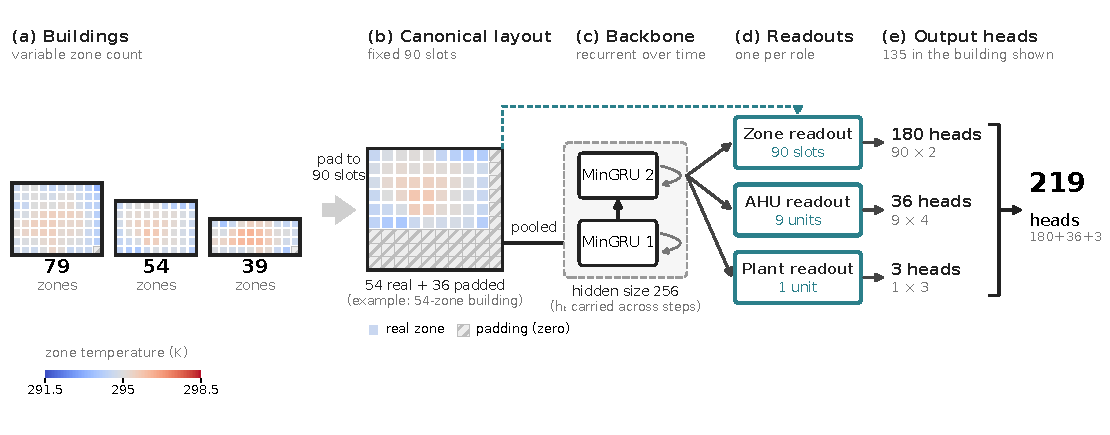
\includegraphics[width=\linewidth]{figures/fig_architecture_v2.pdf}
\caption{Architecture of the shared control policy. (a) Three of the six training buildings (79, 54, and 39 zones), zones shaded illustratively by temperature on a shared scale. (b) State slotization: buildings map into 90 fixed zone slots (e.g., 54 active zones and 36 zero-padded slots), 9 AHU slots, 1 plant slot and 1 global slot, 983 values in all. (c) An 80-value pooled summary enters a two-layer recurrent backbone (256 hidden units per layer) that carries one state across steps; each readout also reads its own local slice, 68 values for a zone, 32 for an air handler and 16 for the plant. (d) Shared readout networks grouped by equipment role rather than individual identity. (e) Multi-head policy: 219 heads, 180 for zones (damper and reheat), 36 for AHUs (supply temperature, static pressure, recirculation, on/off) and 3 for the central plant; the pictured building uses 135, and a head a building does not have is masked.}
\label{fig:arch}
\end{figure}

An 80-value pooled summary of that vector (zone and air-handler statistics, plant state, equipment presence, time and occupancy) enters two minimal-GRU layers of 256 hidden units \citep{feng2024rnn}, so the building carries one recurrent state across steps that every slot reads. Each slot's readout combines that state with role-specific local features. For a zone these are its own seven values (temperature, the two setpoint deficits, the heating setpoint, the damper and reheat echoes and presence), the rectified part of each deficit, the eight sensor and echo values of its air handler, and the four sibling entries of every slot in its group, its own included, so a zone is conditioned on its neighbors without a learned attention layer; with the eleven delay features of Appendix~C, a zone reads 68 values, an air handler 32 and the plant 16. Air-handler slots read their own eight values and statistics aggregated over their zones, plus the plant's two loop values. Zone slots also carry a four-hour ring (48 steps) of their own temperature and comfort deficit, from which the history features of Appendix~C are computed.

One readout is shared by every slot of the same role (zone, air handler, plant) rather than learned per zone \citep{zaheer2017deepsets}, so the whole network is 453K parameters shared by all 30 training scenarios. Each zone readout adds a shared 32-unit tanh branch with a zero-initialized output. The slot layout has 219 heads; a building masks the ones it does not have and commands between 75 and 209 of them. The critic reads the same trunk state and no input the actor does not see, and it is a state baseline rather than an action-dependent one \citep{tucker2018mirage}. One parameter set therefore serves every zone, air handler and plant in every building.

\subsection{Bounded Action Parameterization and Policy Optimization}

\subsubsection{Admissible control via bounded Beta distributions}
\label{sec:beta_head}

To control continuous physical actuators without post-hoc clipping or boundary artefacts, each active head outputs a bounded Beta distribution rather than a standard Gaussian. The policy runs on a padded interface of 256 continuous and 16 discrete heads. It uses 219 continuous heads and no discrete head: every on/off command in the environment's hybrid action space (Table~\ref{tab:interface}) is a continuous Beta head read as on when $a > -0.5$, so its discrete half is never used. A building masks every head it does not have. Each head therefore models a Beta distribution over $(0,1)$ \citep{chou2017beta} and emits
\[
a = 2x - 1, \qquad x \sim \operatorname{Beta}(\alpha, \beta);
\]
$a$ is mapped affinely to the range of a continuous command.
We compute the shape parameters from the network outputs $u$ and $v$ as
\[
\alpha = \operatorname{softplus}(u) + 0.5, \qquad \beta = \operatorname{softplus}(v) + 0.5.
\]
The $0.5$ floor lets the density form a central mode ($\alpha,\beta>1$) or a bimodal U-shape ($\alpha,\beta<1$), so a damper can be held firmly open or shut. To prevent entropy from vanishing during training, we cap the sum $\alpha+\beta$ at 12: whenever it would exceed 12, both parameters are rescaled by $12/(\alpha+\beta)$, which preserves the mean $\alpha/(\alpha+\beta)$ while bounding policy certainty. Because every sample is natively bounded, all emitted actions are admissible by construction: no external filtering, clipping or projection sits between the policy and the plant (Appendix~D).

\subsubsection{Multi-head PPO and horizon scaling}

Optimizing up to 209 actuators at once creates a failure mode for standard policy-gradient updates: a joint ratio lets large steps on a few heads hide behind near-zero shifts on the others. We remove this cross-head interference by decoupling the PPO clipping objective across individual control slots \citep{han2019dimension}. Each active head $h$ keeps its own importance ratio at the stored sample,
\[
r_h(\theta) = \frac{\pi_\theta(x_h \mid s)}{\pi_{\theta_{\mathrm{old}}}(x_h \mid s)}.
\]
Each ratio is clipped independently to $[0.8, 1.2]$, that is $\epsilon = 0.2$, and the surrogate sums these clipped objectives over the building's active heads, $\mathcal{H}$,
\[
\mathcal{L}^{\mathrm{CLIP}}(\theta) = \hat{\mathbb{E}}_t\left[\,\sum_{h\in\mathcal{H}} \min\left(r_{h,t}(\theta)\hat{A}_t,\ \operatorname{clip}\left(r_{h,t}(\theta),\, 1-\epsilon,\, 1+\epsilon\right)\hat{A}_t\right)\right].
\]

To stabilize learning across buildings with widely differing baseline returns, advantages are standardized over the entire rollout buffer. With $\gamma = 0.99$ and $\lambda = 0.95$ the credit horizon is about 1.4 hours \citep{schulman2016gae}, which covers the hourly tariff step and the first part of the thermal response, so a price spike attributes credit to the decision that caused it. The policy updates with Adam under a global gradient-norm cap of 0.5, a value coefficient of 0.5, an entropy bonus of 0.001 and a single shared learning rate. We use no reward shaping, potential function or auxiliary objective: the optimization gradient is the competition score.

\subsubsection{Occupancy-weighted zone critics}

To direct credit locally without hundreds of separate networks, we split the reward into per-zone streams,
\[
r_{z,t} = 0.6\,p_{z,t} - 0.2\,s_{z,t}E_t - 0.2\,s_{z,t}C_t, \qquad s_{z,t} = \frac{o_{z,t}}{\sum_{z'} o_{z',t}},
\]
where $p_{z,t}$ is zone $z$'s productivity regret and $E_t$, $C_t$ the building's energy and carbon. The weights are the score's own, so the streams redistribute $r_t$ and add no term. Costs are allocated by occupancy share $s_{z,t}$, and the allocation conserves on occupied steps: the streams sum to the building-level reward, while an empty building reduces every stream to zero. Those steps are not lost: the building-level value is trained on the full return, and the air-handler and plant heads keep the building advantage.

The critic mirrors it: on the pooled representation, the value network outputs one building-level evaluation and 90 zone evaluations. The 90 share one value loss, averaged over batch steps and the 90 slots, and their advantages use generalized advantage estimation (GAE). Each zone head is therefore guided by a local advantage, giving fine credit across dozens of zones in one compact network.

\subsection{Training Configuration}

\textbf{Scenarios and parallel environments.} Training spans 30 scenarios: six building topologies crossed with five diverse climates (Atlanta, Denver, Fairbanks, Phoenix and Singapore). We run 32 parallel environments per scenario (960 total), collecting 288 steps per worker to yield 276,480 transitions per policy update. Episode starts are staggered per environment, and the scenarios carry different months.

\textbf{Objective, budget and precision.} Training optimizes the raw 3C reward of Section 3.1 without modification. The reported policy starts from a fresh random initialization (seed 75) and runs for 199,895,040 environment steps, 723 rollouts, with the learning rate annealed linearly from $10^{-4}$ to zero over that same budget, so the reported checkpoint sits at the end of the anneal, with a step size of $4\times10^{-7}$. Adam \citep{kingma2015adam} updates minibatches of 2,304 with four epochs per rollout, the batch design of \citet{andrychowicz2020matters}. The reported run trains on the double-precision solve, as does every score in this paper. A single-precision solve exists as an opt-in speed experiment and is not used here: it moves the observation by about $1.2\times10^{-4}$ against the double-precision reference, ten orders of magnitude above the default path's $2\times10^{-14}$, which is enough to change the reward the policy is trained on (Appendix~A.4). One 46 GB NVIDIA L40S sustains about 12K environment steps per second, so the full run takes roughly 4.6 hours (Appendix~A.3 and Appendix~E).

\section{Results}

Five policies appear in every comparison. \textbf{PID} is the water-based controller the benchmark ships. \textbf{SAC} is the learned baseline: a 50M off-policy run on the same contract, actor and scenarios, with the bounded Beta action head. \textbf{Long} is the earlier 30-scenario PPO run, a 1.5B-step budget with no linear anneal, stopped at 507.6M steps and best at 89.6M; \textbf{Mid} and \textbf{Final} are the 159.3M and 199.1M saves of the later annealed 200M run, and Final is the policy this paper reports. Two held-out sets are scored and never pooled: 90 months over five buildings, with two of them and the Minneapolis climate never trained, and a 54-month extension over the three shipped buildings missing from the first set, on the same 18 windows.

\subsection{The Score, the Terms and the Two Budgets}

\begin{table}[h!]
\centering
\small
\setlength{\tabcolsep}{4.0pt}
\begin{tabular}{@{}lrrrrrrr@{}}
\toprule
 & steps (M) & comfort & energy & carbon & 90 months & 54 months & public \\
\midrule
PID & -- & 0.0326 & 0.0078 & 0.0057 & 0.0461 & 0.0437 & 0.0640 \\
SAC & 50.1 & 0.0262 & 0.0048 & 0.0028 & 0.0338 & 0.0229 & 0.0252 \\
Long & 89.6 of 507.6 & 0.0137 & 0.0059 & 0.0057 & 0.0253 & 0.0192 & 0.0182 \\
Mid & 159.3 of 199.9 & 0.0080 & 0.0054 & 0.0051 & 0.0185 & 0.0112 & \textbf{0.0175} \\
Final & 199.1 of 199.9 & \textbf{0.0070} & \textbf{0.0051} & \textbf{0.0044} & \textbf{0.0165} & \textbf{0.0098} & 0.0294 \\
\bottomrule
\end{tabular}
\vspace{4pt}
\caption{The five policies on the 90-month set, the 54-month extension and the public leaderboard. The three terms are those of the reward in Section~3.1 with its sign removed, so they sum to the 90-month score; zero is the ideal and lower is better.}
\label{tab:score}
\end{table}


Final scores 0.0165 on the 90 months, 64\% below PID's 0.0461, 35\% below Long's best save and 11\% below Mid, and it is lower than PID on 89 of the 90 months; the exception is \texttt{train\_3}/\texttt{fairbanks\_6}, 0.0459 against 0.0410. The learned baseline does not reach it: at 50M the Beta-head SAC is 0.0338, 27\% below the controller and twice PPO, and 0.0229 on the 54 months; the earlier 200M run used a tanh-Gaussian head (Appendix~I). On the 54-month extension Final is 0.0098, 78\% below PID, 49\% below Long and 13\% below Mid, lower on all 54. Mid takes the public leaderboard, 0.0175 against Long's 0.0182, SAC's 0.0252, Final's 0.0294 and PID's 0.0640: the public split (Appendix~F) prefers Mid and the SAC arm to the final save, while the 90 and 54 months and all five buildings prefer Final.


The score is the sum of three terms, and Final's gain is mostly comfort: 0.0070 against 0.0326 for PID, 0.0137 for Long and 0.0080 for Mid, while energy falls from 0.0078 to 0.0051 and carbon from 0.0057 to 0.0044. Comfort is the largest term and the largest fall in every comparison, so no term is bought with another: the learned baseline's comfort also falls below the controller's, 0.0262 against 0.0326, as do its energy and carbon (Table~\ref{tab:score}, Figure~\ref{fig:scores}a).

\begin{figure}[t]
\centering
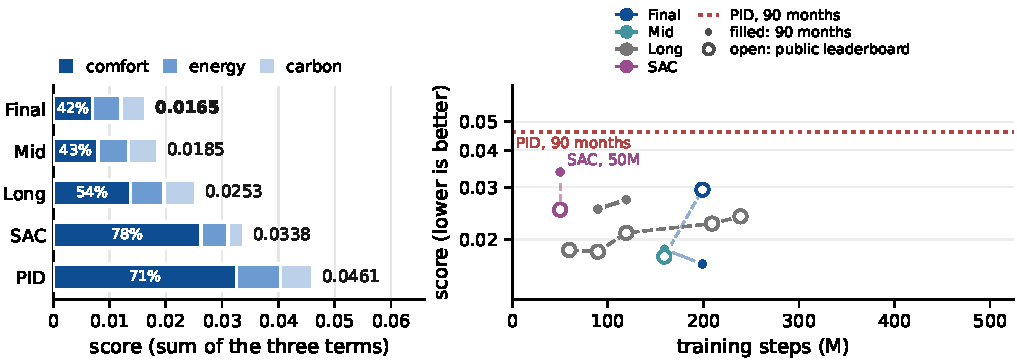
\includegraphics[width=\linewidth]{figures/fig_results_scores_v3.pdf}
\caption{The five policies. (a) The 90-month score as the sum of its three terms, printed at the bar end; comfort is the largest term in every bar. (b) Score against training steps on the 90 months (filled, solid) and on the public leaderboard (open, dashed where a policy has several saves), each policy in its own color; the SAC 50M arm is filled on the 90 months and open on the public split, the two joined by a dashed link. Long is best at 89.6M on both and its public score rises afterwards; the later run improves to 199.1M on the 90 months, while its public score is best at 159.3M. The dotted line is PID on the 90 months, comparable only to the filled series.}
\label{fig:scores}
\end{figure}

\FloatBarrier

\subsection{By Building and by Climate}

Final is below Mid, Long, SAC and the controller on every building and every climate: its building scores run from 0.0078 on \texttt{train\_2} to 0.0443 on \texttt{train\_3}, and its climate scores from 0.0112 in Phoenix to 0.0184 in Fairbanks. The two buildings never trained behave like the rest: on \texttt{train\_6} Final is 0.0126 against PID's 0.0491, and on \texttt{train\_3} 0.0443 against 0.0689; the 40 months of the unseen Minneapolis climate are 0.0180 against 0.0519. SAC does not: on the three buildings it trained on it is below the controller (0.022, 0.021, 0.019 against 0.035, 0.038, 0.039), and on the unseen pair it wins one and loses the other (0.026 against 0.049 on \texttt{train\_6}, 0.081 against 0.069 on \texttt{train\_3}).

\begin{figure}[h]
\setlength{\abovecaptionskip}{2pt}
\centering
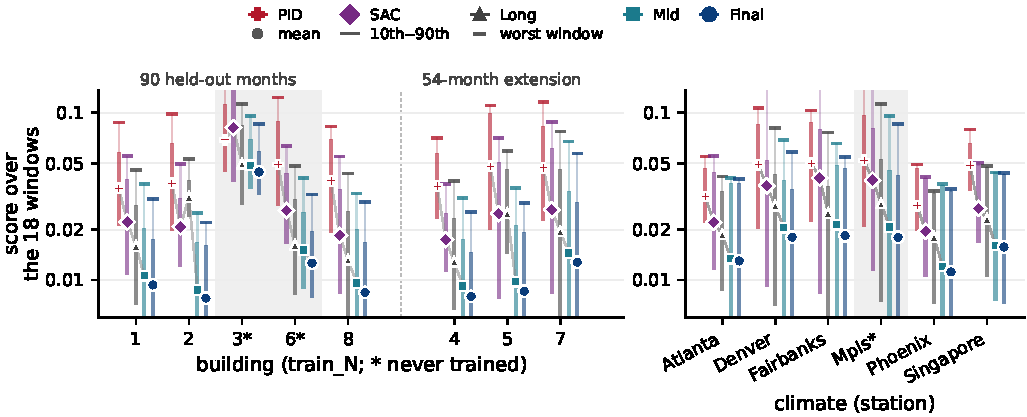
\includegraphics[width=\linewidth]{figures/fig_results_breakdown5.pdf}
\caption{Every building and every climate, five policies. The dot is the mean over the 18 held-out windows, the line the 10th to 90th percentile and the tick the worst window; lower is better. Left: the 90-month set; right: the 54-month extension. A star marks an unseen building or station, and each policy keeps its color and marker.}
\label{fig:breakdown}
\end{figure}

Final's worst window is 0.0855, against 0.1131 for Long and 0.1625 for the controller. \texttt{train\_3} owns all five of its worst months and a fifth of the total (Appendix~F); its 47\% in-band share against 84--98\% elsewhere (Appendix~H) is the residual, not a policy-wide comfort failure. Building identity explains 74\% of the spread in the score, the weather window 22\% and the interaction 4\%, against 19\% and 72\% for the controller (Appendix~G).

On the 54-month extension the buildings are three it trained on. Final is 0.0098 against 0.0437 for the controller and 0.0229 for SAC, lower on all 54; against Long comfort falls 82\%, energy 22\% and carbon 29\%, leaving 14\%, 39\% and 46\%. On the 90 months, occupied zone-steps sit in band 84--98\% on four buildings and 47\% on \texttt{train\_3}; comfort is 42\% of Final's score there, energy 31\% and carbon 27\%.

\subsection{By Time of Day and by Month}

Every policy peaks at 06:00, because the building's schedule does, and that peak belongs to the building, not the controller: PID costs 3.2$\times$ Final at that hour. The gap is not made at 06:00: half (49\%) comes from the six morning hours that follow, 28\% from the afternoon and 19\% from the evening, so the advantage grows with occupied time, not at the switch-on (Appendix~H).

Night is the only part where Final loses to the controller, 0.0045 against 0.0037, and that loss is the price of the morning. On day 0 it burns 44 to 294\,kWh of gas, 57--93\% of it in the last six hours before comfort starts, so the building is in band when occupancy begins, while the controller holds the setpoint through the empty night and pays when people arrive. It saves not by switching equipment off but by choosing when the building is conditioned.

Weekends are 29\% of the steps and 0.2\% of the electricity, because Final lets empty buildings drift, at 0.0001 per step by day and 0.0003 by night, yet they carry only 6\% of the gain: the saving is in the occupied day. By month, Final is lowest in all ten, from 0.033 in January to 0.009 in August (Figure~\ref{fig:time}b). The residual accumulates over the month: \texttt{train\_3} degrades by $3.8\times10^{-4}$\,K per day, about 0.011\,K a month, four times \texttt{train\_6} and seven times \texttt{train\_1}, a creep on the largest plant rather than an hourly spike (Figure~\ref{fig:time}).

\begin{figure}[h]
\setlength{\abovecaptionskip}{2pt}
\centering
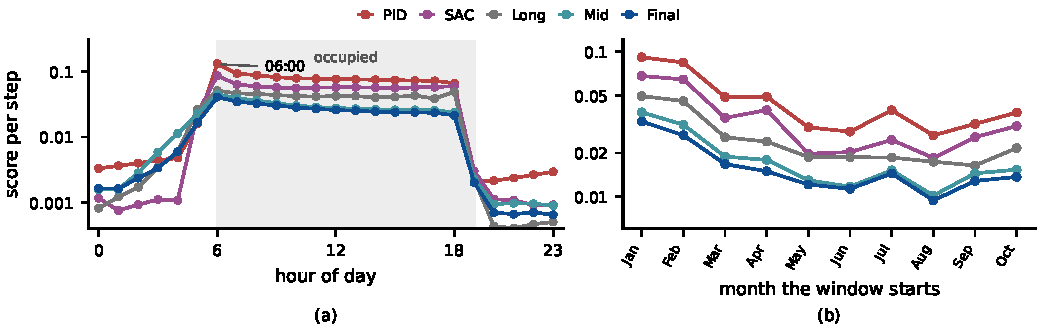
\includegraphics[width=0.8\linewidth]{figures/fig_results_time4.pdf}
\caption{The same recording by hour and by month. (a) Score per step by hour of day, on a log scale; the shaded band is the occupied window, and 06:00 is the most expensive hour for every policy. (b) The month each window starts, January to October. Lower is better throughout.}
\label{fig:time}
\end{figure}


\section{Conclusion}
\label{sec:conclusion}

One shared 453K-parameter PPO policy, trained once across six buildings and five climates and evaluated across eight buildings and six stations, scores 0.0165 on 90 held-out months and 0.0098 on a further 54, against 0.0461 and 0.0437 for the shipped controller. It uses neither model-based control, which inherits the error of the model calibrated for each building, nor rule-based control, which inherits the reach of its rules: its behavior depends on the \textbf{reward alone}.

An off-policy Soft Actor-Critic arm, on the same scenarios, input, seed and 50M budget, separates the action head from the learner. Replacing its Gaussian head with the bounded Beta head takes it from 0.0457 to 0.0338 on the 90 months, below the controller and still twice the reported 0.0165, and from 0.0644 to 0.0261 on one unseen building; every building improves (Appendix~I). \textbf{The head is necessary, not sufficient}: SAC still loses the other unseen building, 0.081 against 0.069, while PPO with the same head adds the rest. The residual is a building, not a season: 74\% of the spread is building identity and 22\% weather, the reverse of the controller's 19/72.

\textbf{Three limits} bound that: one seed, since two seeds at 50M differ by 6\%; ablations at 50M on four scenarios; and training only on the competition's shipped buildings.

\textbf{Future work}: replicate on a \textbf{patched} release of the simulator, run multi-seed training and evaluation, and converge in fewer steps.


\clearpage
\bibliographystyle{unsrtnat}
\nocite{*}
\bibliography{references}

\clearpage
\appendix

\section{Simulator, Validation and Throughput}
\label{app:sim}

\subsection{The Port}
\label{app:port}

The port replaces the finite-difference thermal network, the convection coupling, the sparse solve, the occupancy model and the reward, so a rollout step is one launch per subsystem and a whole update is capturable as a graph. The physics is not approximated: same cells, same boundary conditions, same solver, and the model is the benchmark's (Section~3.1).

\subsection{Validation}
\label{app:validation}

\begin{table}[h!]
\centering
\small
\begin{tabular}{@{}lll@{}}
\toprule
check & comparison & result \\
\midrule
reset observation & port vs reference, per scenario & 0 differing values \\
observation, every step & port vs reference, 30 scenarios, 8{,}640 steps & 0 differing values \\
reward, every step & port vs reference, same runs & 0 differing values \\
thermal solve & port vs CPU replay & differs by about $2\times10^{-14}$ \\
canonical slot map & slots used vs native action count & equal for all six buildings \\
action mask & active heads vs present slots & equal \\
episode length and terminals & port vs reference & equal \\
\bottomrule
\end{tabular}
\vspace{4pt}
\caption{The port against the reference Python implementation. The first three rows are exact comparisons, value by value; the fourth is the only place the two differ.}
\label{tab:app_validation}
\end{table}

Only the solve differs, in the summation order, by about $2\times10^{-14}$. Everything the gateway hands the policy and everything the policy is paid is reproduced exactly, which is what makes it legitimate to score an episode on the GPU.

\subsection{Throughput}
\label{app:throughput}

\begin{table}[h!]
\centering
\small
\begin{tabular}{@{}llrr@{}}
\toprule
configuration & hardware & agents & steps/s \\
\midrule
30 scenarios, 32 agents each & NVIDIA L40S, 46\,GB & 960 & 12.0K \\
4 scenarios, 64 agents each & NVIDIA RTX 3090, 24\,GB & 256 & 6.2K \\
reference Python, 12 CPU cores & AMD Ryzen 5700F & 12 & 145 \\
\bottomrule
\end{tabular}
\vspace{4pt}
\caption{Measured environment steps per second, double-precision physics in every row. The reported run uses the 960-agent L40S row.}
\label{tab:app_throughput}
\end{table}

\subsection{Build and Run}
\label{app:build}

Everything is built and executed inside the \texttt{pufferai/puffertank:5.0} image. The reported run used one frozen executable whose digest is recorded with its checkpoints, and its data archive is verified at start-up; a mismatch aborts rather than trains. Evaluation always uses the double-precision path. A single-precision solve exists as an opt-in speed experiment; it is not used for training here either, because its observation differs from the double-precision reference by about $10^{-4}$ and the reward a policy would be trained on would not be the reward this paper reports.

\section{The Input Contract}
\label{app:contract}

The policy never sees a building's own observation vector. It sees this one: 90 zone slots of 9 values, 9 air-handler slots of 16, one plant slot of 10 and one global slot of 19. Zone slot $s = 10k + j$ is the $j$-th zone served by air handler $k$, with handlers in numeric id order and zones in the order their temperature sensor first appears. Slots past a building's counts are zero, which is what makes the vector comparable across buildings; every slot except the global one starts with a presence flag, so a zero there means ``this equipment does not exist'' rather than ``this equipment reads zero''. A slot keeps its width in every building, so an offset always means the same thing. No PID or rule-based controller is used in the policy or in its training loop.

\begin{figure}[h!]
\centering
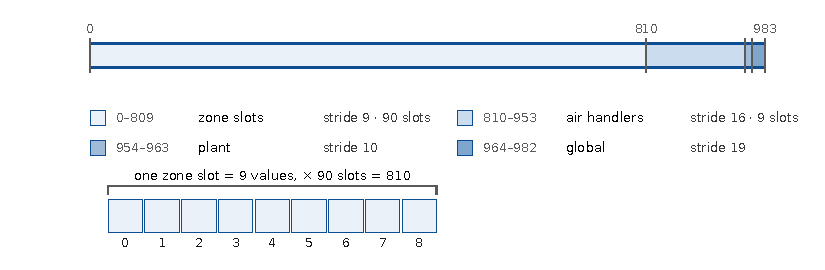
\includegraphics[width=0.95\linewidth]{figures/fig_appendix_slots.pdf}
\caption{The 983-value vector as an address map (top) and as one slot (bottom). Offsets run 0--809 for the 90 zone slots, 810--953 for the 9 air-handler slots, 954--963 for the plant and 964--982 for the global slot, and the legend gives each group's stride. The lower row expands a single zone slot; the numbers under it are positions in the slot, and Table~\ref{tab:app_zone_values} lists the values the policy reads at those positions.}
\label{fig:appendix_slots}
\end{figure}

\subsection{Zone Slots}
\label{app:zone}

\begin{table}[h!]
\centering
\small
\begin{tabular}{@{}rlcl@{}}
\toprule
\# & value & scaling & source \\
\midrule
0 & presence & $1/0$ & equipment map \\
1 & zone air temperature & $(T-295)/5$ & sensor \\
2 & heating setpoint shortfall & $(T-H_s)/2$ & sensor and setpoint \\
3 & cooling setpoint headroom & $(C_s-T)/2$ & sensor and setpoint \\
4 & heating setpoint & $(H_s-294)/3$ & setpoint \\
5 & damper position & $2D-1$ & command echo \\
6 & reheat valve & $2R-1$ & command echo \\
\bottomrule
\end{tabular}
\vspace{4pt}
\caption{The zone slot: seven values, at positions 0--6 of the nine-value slot. $T$ is the zone temperature, $H_s$ and $C_s$ its heating and cooling setpoints, $D$ and $R$ its damper and reheat commands.}
\label{tab:app_zone_values}
\end{table}

\subsection{Air-Handler, Plant and Global Slots}
\label{app:ahu}

The gateway supplies twelve harmonics per family; the canonical layout keeps the first four sine and the first four cosine of each, sixteen values in all, which is the ``16 retained'' line of Table~\ref{tab:interface}.

One choice in this layout is measured rather than assumed: the comfort deficits are stored as magnitudes, not as signed values. The signed variant, which would let a zone that is too hot excite the cold shortfall that opens its reheat valve, costs 33\% of the ten-month panel and is worse at all six saves.

\begin{table}[h!]
\centering
\small
\begin{tabular}{@{}rlcl@{}}
\toprule
\# & value & scaling & source \\
\midrule
0 & presence & $1/0$ & equipment map \\
1 & outdoor air temperature & $(T_{oa}-283)/15$ & sensor \\
2 & supply-air static pressure & $P/1000$ & sensor \\
3 & supply-air flowrate & $F/10$ & sensor \\
4 & outdoor-air flowrate & $F/10$ & sensor \\
5 & supply-air temperature setpoint & $(T_s-295)/5$ & setpoint \\
6 & recirculation & $2R-1$ & command echo \\
7 & cooling request count & $C/10$ & equipment \\
8 & run command & $2u-1$ & command echo \\
\bottomrule
\end{tabular}
\vspace{4pt}
\caption{The air-handler slot: nine values, at positions 0--8 of the sixteen-value slot. $T_{oa}$ outdoor air temperature, $P$ static pressure, $F$ flowrate, $T_s$ supply-air temperature setpoint, $R$ recirculation, $C$ cooling request count, $u$ run command.}
\label{tab:app_ahu}
\end{table}

\begin{table}[H]
\centering
\small
\begin{tabular}{@{}rlcl@{}}
\toprule
\# & value & scaling & source \\
\midrule
\multicolumn{4}{@{}l}{\emph{plant slot (10)}} \\
0 & presence & $1/0$ & equipment map \\
1 & supply-water temperature & $(T-330)/20$ & sensor \\
2 & supply-water temperature setpoint & $(T-330)/20$ & setpoint \\
3 & differential pressure & $P/10$ & sensor \\
4 & differential pressure setpoint & $P/10$ & setpoint \\
5 & run status & $2r-1$ & status \\
6 & heating request count & $/10$ & equipment \\
\multicolumn{4}{@{}l}{\emph{global slot (19)}} \\
0--3 & hour harmonics, sine & as supplied & calendar \\
4--7 & hour harmonics, cosine & as supplied & calendar \\
8--11 & day-of-week harmonics, sine & as supplied & calendar \\
12--15 & day-of-week harmonics, cosine & as supplied & calendar \\
16 & comfort mode now & $0/1$ & schedule \\
17 & comfort mode in 60 minutes & $0/1$ & schedule \\
18 & building occupancy & occupants & sensor \\
\bottomrule
\end{tabular}
\vspace{4pt}
\caption{Plant and global slots. The plant slot has ten positions and the seven listed are the ones the policy reads; the global slot carries the only calendar information the policy receives and the only building-wide occupancy information.}
\label{tab:app_plant}
\end{table}

\subsection{Field Identifiers, Collisions and Missing Values}
\label{app:fields}

A field identifier is the device id joined to the measurement name. When that string already belongs to another pair the gateway appends \texttt{\_1}, so an identifier is unique but not parseable by pattern; the canonical map is built from the identifier list in device order, never by matching a regular expression. A missing measurement is filled from the previous observation rather than zeroed, because a zero in a temperature field is a plausible temperature and would silently corrupt the features. Neither rule is learned; both are applied identically at training and at evaluation.

\subsection{The Reward's Schedules}
\label{app:reward}

The comfort term is the only unbounded one. A zone that sits far outside its band costs more than the entire energy and carbon bill of a good month, which is why the tail of the score, not its mean, is the quantity a practitioner should watch.

Every value the policy reads is named and scaled, and the schedule the reward is computed from is the benchmark's own rather than one we chose.

\section{Delay Features and the Memory}
\label{app:delay}

\begin{figure}[h!]
\centering
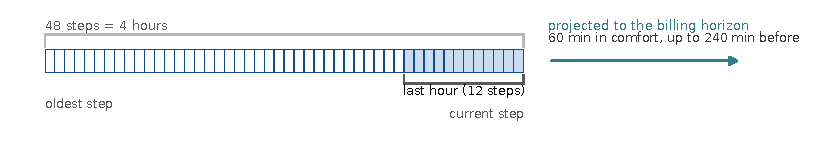
\includegraphics[width=0.8\linewidth]{figures/fig_appendix_memory.pdf}
\caption{The per-zone memory. Each zone keeps its last 48 temperature and deficit samples, four hours at five minutes per step, and projects its own trajectory forward to the moment the delayed reward is billed: sixty minutes while comfort is active, up to four hours while the building waits for occupancy.}
\label{fig:appendix_memory}
\end{figure}

A setpoint change is paid for hours later, and the thermal mass that delays the bill is not in the observation. Each zone therefore carries a short history of itself and a projection of where it is heading, both computed from the gateway vector alone.

\subsection{The Ring}
\label{app:ring}

Each zone slot carries a ring of 48 samples of its own temperature and of its distance outside the comfort band. The ring is empty at the first step and fills as the episode runs, so the history-derived features become informative once one hour of history exists; the four entries taken from the observation itself are valid from step one.

\subsection{The Eleven Features}
\label{app:features}

\begin{table}[h!]
\centering
\small
\setlength{\tabcolsep}{4pt}
\begin{tabular}{@{}rlp{0.5\linewidth}c@{}}
\toprule
\# & feature & definition & clip \\
\midrule
0 & minutes to comfort start & $t_{\text{start}}/180$ & -- \\
1 & minutes to comfort end & $t_{\text{end}}/180$ & -- \\
2 & next-day flag & comfort starts more than a day away & 0/1 \\
3 & outdoor temperature change & $\Delta T_{oa}/2$ over one step & -- \\
4 & current deficit & band distance $/5$ & -- \\
5 & mean deficit over the last hour & mean of 12 samples $/5$ & -- \\
6 & mean deficit over the ring & mean of up to 48 samples $/5$ & -- \\
7 & temperature slope & K per hour, from the ring & -- \\
8 & mean temperature over the ring & $(\bar T-295)/5$ & -- \\
9 & deficit projected to billing & band distance of $T+\text{slope}\cdot h$ & $\le 10$ \\
10 & fan path & damper $\times(H_s-T)/5$, reheat $<0.3$, supply $\le T$ & $\le 10$ \\
\bottomrule
\end{tabular}
\vspace{4pt}
\caption{The engineered features appended to each zone slot, after the seven of Table~\ref{tab:app_zone_values}, the eight air-handler values it inherits and the two rectified setpoint deficits. The last two are the ones that close the delay.}
\label{tab:app_features}
\end{table}

Feature 9 is the delay closed in the state: $h$ is 60 minutes while comfort is active and $\min(t_{\text{start}},240)$ while it is not, so the feature asks ``how far out of band will this zone be when the reward is charged?'', not ``how far out is it now''. Feature 10 is the second half of the same argument: a damper held open on a zone that is already below its heating setpoint, with the reheat valve closed and supply air no warmer than the room, means the fan is doing the heating and the electricity for it is billed later. Both are clipped at ten so a single frozen zone cannot dominate the input.

What these features are worth is measured, and the honest answer is split. The critic was given its own eight-number summary of the same quantities, and removing it improves the ten-month panel by 9\% and is better at all six saves: presented to the critic, the delay numbers add nothing, which is consistent with the earlier finding that the critic ranks time well and rooms poorly. The actor keeps the projection and the fan path, because those are the features the action is chosen from, and the loop is closed through the reward. What we have not done is isolate the actor's block with a single-flag arm at the final recipe, and we say so rather than implying a measured gain for it. The ring and the projection are therefore described here as a design that encodes the delay, not as a component with an attributable score contribution.

\subsection{What Resets at an Episode Boundary}
\label{app:reset}

The ring, its sample count and the outdoor-temperature memory are cleared at every episode boundary. The comfort schedule and occupancy are not, because they come from the gateway vector. Nothing is carried across scenarios, so the policy cannot recognize a building from its history.

Every number in the input is named, scaled and reproducible from the gateway vector, and the two quantities that close the delayed reward, the projected deficit and the fan path, are computed from that vector alone, reset with the episode, and clipped so that one zone cannot dominate.

\section{The Action Distribution and the Optimizer}
\label{app:action}

Up to 219 heads draw from one trunk, so two properties decide whether the arrangement trains at all: whether a head can sit at the end of its range without losing the gradient that would bring it back, and whether one head can be corrected without moving the others. Both are properties of the distribution and of the update rule rather than of the network's width, and both were measured at the final recipe, one change per arm.

\begin{figure}[h!]
\centering
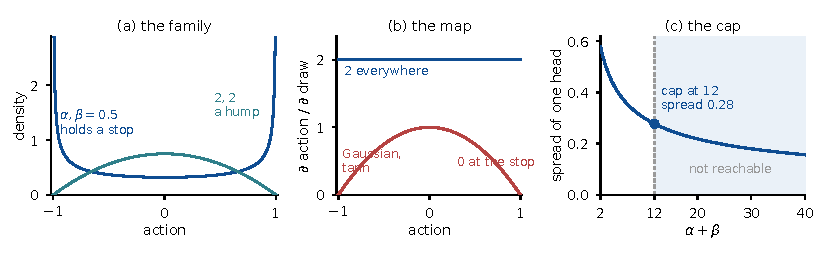
\includegraphics[width=0.95\linewidth]{figures/fig_appendix_beta.pdf}
\caption{The shape of one control head. (a) A Beta with both parameters below one puts its mass at the two stops, which is how a damper is held shut or a valve held open; with both above one it is a hump, which is how a command tracks a setpoint. (b) The tanh map that a squashed Gaussian needs has derivative $1-a^2$, which is 0.10 at nine tenths of the range and 0 at the stop; the Beta's affine map has the same sensitivity everywhere. (c) The spread of a head falls as $\alpha+\beta$ rises, so without a cap the policy can make a head arbitrarily certain; the cap at 12 holds the spread at 0.28 action units.}
\label{fig:appendix_beta}
\end{figure}

\subsection{A Support That Is the Actuator Range}
\label{app:support}

The support argument is Section~3.4.1. We kept the parameterization for a behavioral reason, not for a score. Our earlier implementation used the squashed Gaussian, settled into a cold operating point and did not leave it; the Beta variant, whose support covers the whole range and whose width can reopen, did. The state belongs to a month, not to the batch: the runs that separated the two were on one cold-demand month (Fairbanks), and in the reported run it appears on a single month, \texttt{train\_1/fairbanks\_1}, which sat at a month score of 5.3 per step for about 60M steps until the anneal moved it. In that state the dampers sit nearly shut, the reheat valves nearly fully open and recirculation at its cap. That observation precedes every arm in this appendix, so it is the motivation and not a measurement.

\subsection{A Cap on Certainty}
\label{app:cap}

The cap rescales both parameters by $12/(\alpha+\beta)$, which lowers the concentration and leaves the mean unchanged (Section~3.4.1). The cap is worth 64\% of the panel. Removing it moves the final score from 0.033 to 0.054, worse at all six saves, and the early panel (2.18 at 10M against 0.273) is the hot-month lock returning: a run that has committed to one operating point so hard that it cannot sample its way out. The cap is not a reward regularizer and does not touch the score; it bounds how certain a head may become, which is a property of the search.

\subsection{One Ratio per Head}
\label{app:ratio}

We use the dimension-wise clip of \citet{han2019dimension}. Standard PPO multiplies the active densities into one ratio and clips that product once, so a head at 1.30 and a head at 0.80 cancel to 1.04 and neither is corrected. Here each head keeps its own ratio, clipped on its own, so the surrogate is a sum over heads rather than a product:
\[
\tilde r_h(\theta) = \mathrm{clip}\!\left(\frac{\pi_\theta(x_h\mid s)}{\pi_{\theta_{\text{old}}}(x_h\mid s)},\ 0.8,\ 1.2\right).
\]
The measured effect is the second largest in Appendix~\ref{app:ablation}: 0.152 against 0.033. The arm without it is ahead at 20M (0.096 against 0.126) and then flat at 0.15 while the unmodified recipe falls to 0.033, a policy that can raise the joint likelihood but cannot repair one zone. Nothing else changes: the reward, the executed action and the physics are the same.

\subsection{An Optimizer That Adapts per Weight}
\label{app:adam}

The earlier recipe ran Muon on the trunk and Adam only on the readout rows, on the argument that an orthogonalized update needs a per-weight correction on the small matrices it feeds. Both halves of that arrangement are measured. Remove the readout Adam while the trunk stays on Muon and the panel moves from 0.033 to 0.049, 48\% worse and worse at every save. Replace Muon with Adam everywhere and drop the split, and the panel moves to 0.029, better at all six saves and 41\% better than the arm that only dropped the split.

In this recipe the split behaves as a compensation rather than a component. Once the trunk's update adapts per weight, the correction it was there to provide has nothing left to correct, and keeping it is worse than dropping it. That mechanism is a conjecture; what is measured is that Adam everywhere is better at the same wall clock, 6{,}018 against 6{,}069 steps per second.

\section{The Training Recipe and Checkpoint Selection}
\label{app:recipe}

The appendix describes three different runs. The ablation arms of Appendix~E.1 and E.2 are sixteen: fifteen change one setting from the unmodified recipe and one makes all the adopted changes at once. Each arm is trained from a fresh random initialization, seed 75, for 50{,}135{,}040 steps on the four-scenario batch (256 agents). The checkpoint study of Appendix~E.3 is the reported run: 199{,}895{,}040 steps annealed to zero over the 30 scenarios, 960 agents, seed 75, and six saves, of which Final is 199.1M and Mid is 159.3M. Long is a separate earlier run, stopped at 507.6M and best at 89.6M. From here, ``the policy'' means Final unless another save is named. The read is the training panel, the mean episode score over the batch's scenarios on whole 8{,}640-step months, evaluated while the policy is still changing; it is a learning-curve statistic, not a frozen score, and not the held-out set.

\subsection{Staggered Episode Starts}
\label{app:stagger}

The largest effect we measured is not a network or an optimizer choice but how the batch samples the calendar. With staggered starts every environment begins its month at its own phase, so a rollout contains many points of the seasonal and weekly cycle at once; with a common start every environment sits at Sunday 06:00 and every update sees a single calendar state.

With a common start every update sees one calendar state, and the arm never recovers: 2.213 against 0.033, worse at every save (Figure~\ref{fig:appendix_ablation}).

\subsection{What Each Change Is Worth}
\label{app:ablation}

\begin{figure}[h!]
\centering
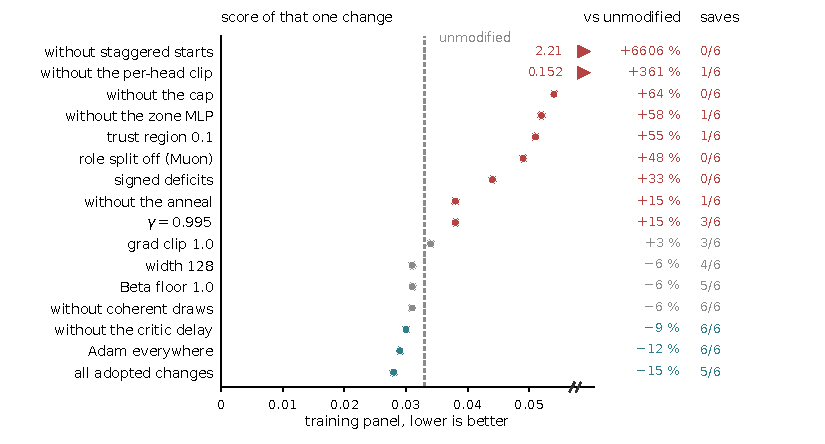
\includegraphics[width=0.72\linewidth]{figures/fig_appendix_ablation.pdf}
\caption{Fifteen single changes to the unmodified recipe and one arm that makes all the adopted changes at once, each trained for 50.1M steps from a fresh initialization. The dashed line is the unmodified recipe at 0.033; a dot is the score with that one change and everything else left alone. Two changes score past the axis and are drawn as arrows with their values. A positive percentage means worse than the unmodified recipe and a negative one better.}
\label{fig:appendix_ablation}
\end{figure}

\begin{figure}[h!]
\centering
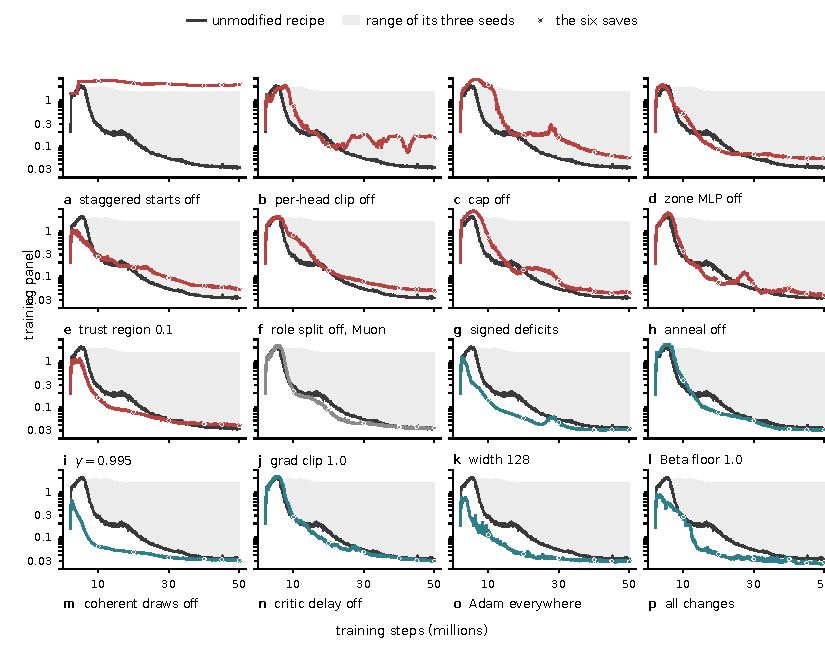
\includegraphics[width=0.98\linewidth]{figures/fig_ablation_A.pdf}
\caption{The curves behind Figure~\ref{fig:appendix_ablation}: each panel repeats one change (colored) against the unmodified recipe (black) and the range of its three seeds (gray); dots mark the six matched saves and the ordinate is logarithmic. Lower is better.}
\label{fig:appendix_curve}
\end{figure}

Figure~\ref{fig:appendix_ablation} ranks the changes by their final value and Figure~\ref{fig:appendix_curve} shows the curves behind that ranking. Three matter more for shape than endpoint: the per-head clip is ahead at 20M then flat at 0.15 while the unmodified recipe reaches 0.033; the cap spikes to 2.18 at 10M and stops at 0.054; and $\gamma=0.995$ learns faster for 30M and converges worse after 40M. A trust region of 0.1 ends at 0.051. The coherence change counts once: zeroing either coherence time gives the same $-6\%$ and the same curve, so the two flags are one mechanism (correlated action sampling, \citealp{hollenstein2023colored}; \citealp{korenkevych2019autoregressive}). The last panel is the recipe adopted for the reported run, trained here on four scenarios: Adam in place of Muon with the role split dropped, coherent draws off, the critic's delay summary removed and the Beta floor at 0.5; it reaches 0.042 at 20M where the unmodified recipe is at 0.126, ends at 0.0280 against 0.0330, and its last five readings stay between 0.026 and 0.028.

\subsection{Checkpoint Selection}
\label{app:selection}

Final is one of six saves of that run. The rule was fixed before the held-out months were scored: take the save with the lowest training panel, and reject a save that lowers the mean only by blowing out the worst zone. The panel is the only signal available while training; the 90 months play no part in the choice.

The panel is a read of a policy that is still changing, which is why the choice matters: it stays between 0.07 and 0.26 for the first 120M steps and falls to 0.011 only after 145M, as the step size decays, so a save at 120M reads eleven times its final value.

The panel falls from 0.244 to 0.011, and the typical worst zone with it (Table~\ref{tab:app_saves}), while the worst single episode stays between 9.6 and 12.8\,K across the six saves, the noise of one window rather than a trend. The last two saves are therefore indistinguishable. We report 199{,}065{,}600 because it is the last save with a complete diagnostic row; the final epoch was logged for the panel only. The panel selects the weights, and the deterministic month reports them.

\begin{figure}[h!]
\centering
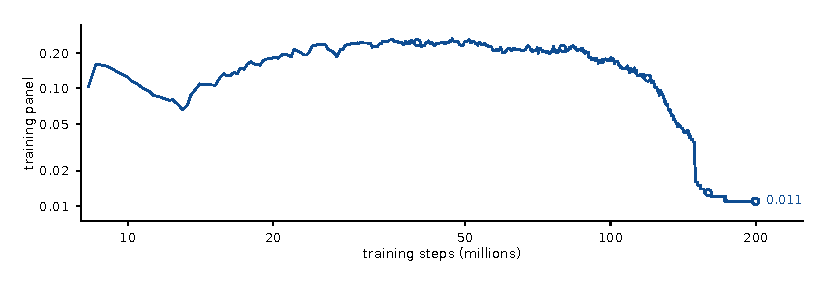
\includegraphics[width=0.90\linewidth]{figures/fig_appendix_curve.pdf}
\caption{The training panel of the reported run's 199.9M steps, one point per rollout, with the six saves marked. The ordinate is logarithmic, so the last decade gets the same room as the first: the panel stays near 0.2 for 120M steps, then falls to 0.011 after 145M as the learning rate decays. It is read over 30 scenarios and is not comparable with the four-scenario panels of Figures~\ref{fig:appendix_ablation} and~\ref{fig:appendix_curve}; the held-out score of the final checkpoint, 0.0165, is a third measurement on different months.}
\label{fig:appendix_panel}
\end{figure}

\begin{table}[h!]
\centering
\small
\begin{tabular}{@{}lrrrr@{}}
\toprule
save (M steps) & training panel & worst episode (K) & worst zone, typical (K) & out of band \\
\midrule
39.8 & 0.2435 & 12.41 & 3.30 & 0.334 \\
79.6 & 0.2177 & 12.77 & 3.28 & 0.309 \\
119.4 & 0.1224 & 11.73 & 2.99 & 0.315 \\
159.3 & 0.0128 & 9.65 & 1.98 & 0.203 \\
199.1 & 0.0109 & 10.07 & 1.96 & 0.236 \\
199.9 & 0.0109 & 11.9 & 1.81 & 0.260 \\
\bottomrule
\end{tabular}
\vspace{4pt}
\caption{The six saves of the reported run, 199{,}895{,}040 steps annealed over the 30 scenarios. ``Worst episode'' is the mean over episodes of the largest zone deviation reached in that episode; ``worst zone, typical'' is the mean over the last logging window of the per-step maximum; ``out of band'' is the fraction of zone-steps outside the comfort band. The last row's diagnostics are the last logged window, one epoch before that save.}
\label{tab:app_saves}
\end{table}

Two limits: the choice uses the training panel, not the held-out months, so the 90-month score is not a selection criterion; and there is one seed, so a difference between arms is not a distribution.

\section{Evaluation, the Metric and the Baseline}
\label{app:eval}

A month is reduced to one number, and the leaderboard to one number over months. For scenario $i$ with $T=8{,}640$ steps,
\[
S_i=\frac{1}{T}\left|\sum_{t=1}^{T}r_{i,t}\right|,\qquad \text{score}=\frac{1}{N}\sum_{i=1}^{N}S_i,
\]
where $r_{i,t}$ is the 3C reward of Section~3.1. Every term of $r$ is non-positive, so the absolute value only changes the sign: the score is the mean loss of one month, zero is the ideal, and the leaderboard is the mean of those losses over the graded months.

\subsection{What the Mean Hides}
\label{app:abs}

The score is one vote per month, not per zone and not a median: a building with 85 zones does not weigh four times one with 30, and a building the policy controls badly arrives at full weight. That makes the mean fragile when a few months are much worse than the rest. Over the 90 months Final's mean is 0.0165 and its median is 0.0094; the five worst months are all \texttt{train\_3}, and they carry a fifth of the total. We report the mean with the per-building and per-climate breakdown of Figure~\ref{fig:breakdown} and the sorted tail of Figure~\ref{fig:appendix_terms}, because a median or a building average would hide that tail.

\subsection{The Deterministic Evaluator}
\label{app:det}

Each scenario is one episode of 8{,}640 steps in double precision, starting at the scenario's own timestamp, with the action set to the mean of each Beta head rather than a sample: no exploration noise, no early termination and no second seed. A scenario therefore has one trajectory, and every spread in this paper is across scenarios, not across runs.

The evaluator writes the observation, the executed action, the reward, its three terms and the per-step diagnostics, and every table in the results section is computed from those recordings rather than from a second episode. The submitted policy, Final's weights in a CPU re-implementation, reproduces the GPU score to within $3\times10^{-4}$ on two held-out months, which is what makes a local month and a graded month the same measurement.

\subsection{The Shipped Controller}
\label{app:baseline}

\texttt{pid\_water} is the benchmark's water-based PID controller: a proportional-integral loop on each zone's temperature error, driving the water valve and the damper, with a supply-water reset. It reads the same observation and it has no term for price or carbon.

\begin{table}[h!]
\centering
\small
\begin{tabular}{@{}lrr@{}}
\toprule
controller & scenarios & score \\
\midrule
\multicolumn{3}{@{}l}{\emph{the 30 shipped scenarios, each controller as supplied}} \\
\texttt{bang\_bang} & 30 & 0.2252 \\
\texttt{pid} & 30 & 0.0674 \\
\texttt{fixed\_setpoint} & 30 & 0.0659 \\
\texttt{pid\_water} & 30 & 0.0541 \\
\multicolumn{3}{@{}l}{\emph{the 90 held-out months this paper scores}} \\
\texttt{pid\_water} & 90 & 0.0461 \\
Final & 90 & 0.0165 \\
\bottomrule
\end{tabular}
\vspace{4pt}
\caption{The shipped controllers on the benchmark's own scenarios, and the two numbers this paper compares. The blocks are different scenario sets: a score may be compared inside a block, never across it.}
\label{tab:app_baseline}
\end{table}

It is the controller the benchmark ships, not one we tuned: every gain is the default. We say so because a tuned PID would be a stronger opponent, and because the claim is only that the learned policy is better than the controller the benchmark supplies. The gap is not uniform. On one window (\texttt{singapore\_4}) the shipped \texttt{fixed\_setpoint} controller scores 0.024 against \texttt{pid\_water}'s 0.108, so the PID is not the best classical controller everywhere, and it is the one we happened to beat by the largest margin.

\subsection{The Public Leaderboard}
\label{app:public}

All five policies have a public score. The public split is the third of the hidden evaluation the competition publishes, 48 scenarios; the other two thirds are private and we do not see them. The scores are the public column of Table~\ref{tab:score}, and every policy is below the controller there. Among the learned policies the split ranks Mid first at 0.0175, then Long at 0.0182, the 50M SAC arm at 0.0252 and Final at 0.0294: Final is last of the four, the reverse of the 90 and 54 months.

The reversal is a property of the split rather than evidence that the final save is worse. A mean over 48 months is more sensitive to a single bad month than a mean over 90, and the only local quantity that orders the two PPO saves the way the split does is the worst-episode excursion, 9.65\,K for Mid against 10.07\,K for Final (Table~\ref{tab:app_saves}); on the 90 months Final is the better of the two. The SAC arm is the sharper case: it is 0.0042 ahead of Final on the split and 0.0173 behind it on the 90 months. The public score is therefore reported beside the local sets and never instead of them, and the policy this paper reports is the last save of the anneal (Appendix~\ref{app:selection}), not the public favourite.


\subsection{A Paired Comparison Against the Controller}
\label{app:paired}

Every scenario is scored once under each policy, so the comparison is paired month by month. Final wins 89 of 90, 54 of 54 and 143 of 144 months; the mean differences are 0.0296, 0.0339 and 0.0312, with 95\% bootstrap intervals of [0.0259, 0.0336], [0.0293, 0.0391] and [0.0282, 0.0344] (exact sign test, $p = 1.5\times10^{-25}$, $1.1\times10^{-16}$ and $1.3\times10^{-41}$; paired $t$ and Wilcoxon agree). All eight building means are positive, 0.0246 to 0.0392. The intervals resample months, not seeds, and the per-building panel of Figure~\ref{fig:breakdown} is the cluster view.

\begin{table}[h!]
\centering
\small
\begin{tabular}{@{}lrrrrr@{}}
\toprule
set & months & mean difference & 95\% interval & won & sign test \\
\midrule
90 & 90 & 0.0296 & [0.0259, 0.0336] & 89/90 & $1.5\times10^{-25}$ \\
54 & 54 & 0.0339 & [0.0293, 0.0391] & 54/54 & $1.1\times10^{-16}$ \\
144 & 144 & 0.0312 & [0.0282, 0.0344] & 143/144 & $1.3\times10^{-41}$ \\
\bottomrule
\end{tabular}
\vspace{4pt}
\caption{Paired differences against the shipped controller, positive when the policy is better. The interval is a 95\% percentile bootstrap over scenarios; the sign test is exact and two-sided.}
\label{tab:app_paired}
\end{table}

\section{Buildings and Climates}
\label{app:buildings}

One set of 453K weights serves eight buildings and six weather stations. Six buildings crossed with five stations, one month per pair, is the training set; the evaluation crosses five buildings with eighteen windows, and two of those buildings and one of those stations never appear in training. Buildings differ in size, plant count, envelope and occupancy; they do not differ in the interface they are written into (Appendix~\ref{app:contract}).

\begin{table}[h!]
\centering
\small
\begin{tabular}{@{}lrrrrrr@{}}
\toprule
building & zones & air handlers & zones per handler & floors & floor area (10$^3$ ft$^2$) & commands \\
\midrule
\texttt{train\_1} & 39 & 4 & 9.8 & 3 & 210 & 97 \\
\texttt{train\_2} & 85 & 9 & 9.4 & 2 & 253 & 209 \\
\texttt{train\_4} & 54 & 6 & 9.0 & 3 & 272 & 135 \\
\texttt{train\_5} & 79 & 8 & 9.9 & 4 & 271 & 193 \\
\texttt{train\_7} & 36 & 4 & 9.0 & 2 & 142 & 91 \\
\texttt{train\_8} & 30 & 3 & 10.0 & 2 & 126 & 75 \\
\midrule
\texttt{train\_3} & 70 & 7 & 10.0 & 3 & 837 & 171 \\
\texttt{train\_6} & 43 & 6 & 7.2 & 2 & 390 & 113 \\
\bottomrule
\end{tabular}
\vspace{4pt}
\caption{The eight buildings. ``Commands'' is the number of actuators the gateway accepts: two continuous per zone, three per air handler and two for the plant, plus one on/off command for each handler and for the pump. The last two rows were generated with their own geometry and materials for the evaluation and were never trained on.}
\label{tab:app_buildings}
\end{table}

\subsection{The Buildings}
\label{app:building_text}

The six trained buildings span 30 to 85 zones, 3 to 9 air handlers, 2 to 4 floors and 126 to 272 thousand square feet of floor area, and the number of continuous commands spans 71 to 209. Occupancy differs by design: 8 to 31 people on average across the five evaluated buildings, and a fixed 36\% of the month carries an occupant in every one of them, so the comfort term is billed on the same share of time whatever the building.

The two generated buildings are not at the ends of the range. They were built with their own materials and geometry and sit in the middle and upper middle of the plant-size range, so the unseen pair is not ``small versus new''.

\subsection{The Climates}
\label{app:climates}

Five stations are trained, from Fairbanks and Denver through Atlanta and Phoenix to Singapore, and Minneapolis enters only at evaluation. Demand is measured in degree-days, the sum over the month of how far the outdoor temperature sits below 18\,$^\circ$C or above 21\,$^\circ$C. Across the 48 months the heating demand runs from 0 to 1182 and the cooling demand from 0 to 475, and the mixed months need both.

Figure~\ref{fig:appendix_climate} is the precise statement of what ``unseen weather'' means here. Nine of the ten scored windows at a trained station fall inside that station's trained range; the tenth, Denver's January window, carries 46\% more heating demand (567 degree-days against a trained maximum of 389) than any Denver month Final saw. Minneapolis has no trained range: eight scored months, no trained month. The two kinds of novelty, a colder month at a known station and a whole new station, are not the same test.

\begin{figure}[h!]
\centering
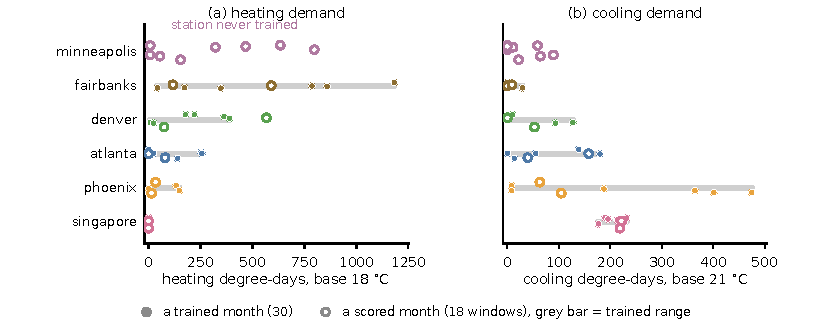
\includegraphics[width=0.95\linewidth]{figures/fig_appendix_climate.pdf}
\caption{The 48 months. Each row is a station; the gray bar is the range of the months trained on there, filled circles are trained months and open circles are scored months.}
\label{fig:appendix_climate}
\end{figure}

\subsection{What Is Held Out}
\label{app:holdout}

Two of the eight buildings, one of the six stations and all 18 windows are held out: every scored window is a calendar month that never appears in the 30 training scenarios. The check is by name as well as by construction: 0 of the 90 scenario names occurs in any training batch (Figure~\ref{fig:appendix_coverage}).

Two limits belong beside that claim. The training set is a design rather than a sample: one month per building-station pair, chosen to cover the year, so the policy never sees two consecutive months at one station. And the evaluation set is a design too, two windows per trained station plus eight for Minneapolis, so its station balance is not the competition's. Both are the right choice for a controlled comparison and neither is a random draw from the year.

\begin{figure}[h!]
\centering
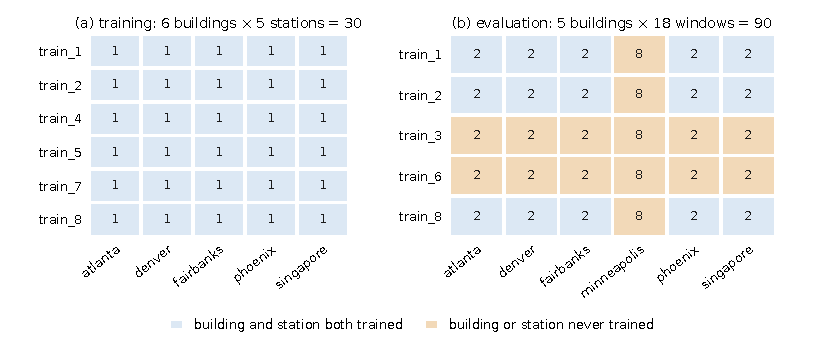
\includegraphics[width=\linewidth]{figures/fig_appendix_coverage.pdf}
\caption{Coverage of the two sets. (a) the 30 training scenarios, one month for each building-station pair. (b) the 90 scored months: five buildings, two windows per trained station and eight for Minneapolis. Orange marks a cell in which the building or the station was absent from training.}
\label{fig:appendix_coverage}
\end{figure}

\subsection{The 54-Month Extension}
\label{app:extension}

The three shipped buildings missing from the 90-month set, \texttt{train\_4}, \texttt{train\_5} and \texttt{train\_7}, are scored on the same 18 windows, 54 months in all. All five policies are scored on them. The extension is never pooled with the 90; the two sets sit side by side in Table~\ref{tab:score}. Per building, the means are 0.0080, 0.0086 and 0.0128 for Final; 0.0092, 0.0098 and 0.0145 for Mid; 0.0129, 0.0252 and 0.0196 for Long; 0.0174, 0.0250 and 0.0264 for SAC; and 0.0365, 0.0478 and 0.0469 for PID. The ordering is the same as on the 90.

\subsection{What the Score Is Made Of}
\label{app:fuel}

Table~\ref{tab:app_fuel} gives the per-building fuel and CO$_2$ for the five buildings of the 90-month set. Against the controller, electricity falls on every building, 73.3 to 45.2\,MWh in total, gas on three of five, 95.6 to 89.1, and CO$_2$ on four of five, 24.6 to 20.6\,t; gas rises in the two largest plants and CO$_2$ in one, so Final's total is not a fuel swap. The Beta-head SAC arm of Appendix~\ref{app:sac} is not a fuel swap either: it burns less gas than both other policies on all five buildings, 45.7\,MWh a month against 89.1 for Final and 95.6 for the controller, takes 4.5\,MWh more electricity than Final, 49.7 against 45.2, and emits 13.2\,t of CO$_2$ against 20.6. It pays 3.7 times Final's comfort cost for that, so its carbon saving comes from heating less, not from moving load to the grid.

\begin{table}[h!]
\centering
\small
\begin{tabular}{@{}lrrrrrrrrr@{}}
\toprule
 & \multicolumn{3}{c}{electricity (MWh)} & \multicolumn{3}{c}{gas (MWh)} & \multicolumn{3}{c}{CO$_2$ (kg)} \\
\cmidrule(lr){2-4}\cmidrule(lr){5-7}\cmidrule(lr){8-10}
building & Final & PID & SAC & Final & PID & SAC & Final & PID & SAC \\
\midrule
\texttt{train\_8} & 2.8 & 6.2 & 2.8 & 9.8 & 17.6 & 5.0 & 2{,}064 & 3{,}802 & 1{,}183 \\
\texttt{train\_1} & 4.7 & 7.5 & 4.7 & 13.5 & 19.3 & 6.3 & 2{,}916 & 4{,}238 & 1{,}612 \\
\texttt{train\_6} & 8.3 & 11.9 & 9.2 & 15.7 & 12.6 & 7.8 & 3{,}668 & 3{,}453 & 2{,}329 \\
\texttt{train\_3} & 21.1 & 33.4 & 24.7 & 29.1 & 24.6 & 15.4 & 7{,}367 & 7{,}766 & 5{,}259 \\
\texttt{train\_2} & 8.3 & 14.3 & 8.3 & 21.0 & 21.5 & 11.1 & 4{,}622 & 5{,}304 & 2{,}838 \\
\bottomrule
\end{tabular}
\vspace{4pt}
\caption{Fuel and CO$_2$ per building over each building's 18 held-out months, from the recorded \texttt{elec\_kwh} and \texttt{gas\_kwh}; the baseline is converted from its recorded cost with the same price and emission schedules, and the SAC columns come from its recording (Appendix~I). Gas rises on \texttt{train\_6} and \texttt{train\_3}, and CO$_2$ on \texttt{train\_6} alone, for Final against the controller; for SAC both fall on all five buildings.}
\label{tab:app_fuel}
\end{table}

The spread of the 90 month scores decomposes on the $5\times18$ building-by-window grid, one month per cell: 74\% of the variance is building identity, 22\% the weather window and 4\% the interaction. There is no replication, so the interaction cannot be separated from noise; it is the residual of the decomposition, not a third mechanism. The same decomposition for \texttt{pid\_water} is 19\% building and 72\% weather, so the controller's month depends mostly on the weather it meets, while Long's two saves, at 89.6M and 119.4M, sit between the two, at 47 to 49\% building and 38 to 49\% weather. The learned policy has largely removed the month-to-month sensitivity, and what remains is a building it has not met rather than a climate it has not met. That reading is what the two sets test: the 54 months hold the buildings and vary only the weather, and score 0.0098 against 0.0165 on the 90.

\section{Behavior and Zones}
\label{app:behaviour}

Final drives 75 to 209 actuators directly. Table~\ref{tab:app_heads} gives what each role does over the 90 months, and every number here comes from the per-step recordings of the 90 months (Section~\ref{app:eval}) and one pass over them.

\begin{table}[h!]
\centering
\small
\setlength{\tabcolsep}{4pt}
\begin{tabular}{@{}lrrrrrr@{}}
\toprule
role & heads & mean & median spread & median step & static months & pinned months \\
\midrule
zone damper & 90 & $+0.01$ & 0.23 & 0.153 & 0\% & 0\% \\
zone reheat & 90 & $-0.11$ & 0.24 & 0.150 & 0\% & 0\% \\
air supply temperature & 9 & $-0.02$ & 0.39 & 0.300 & 0\% & 0\% \\
static pressure & 9 & $-0.65$ & 0.15 & 0.060 & 0\% & 0\% \\
recirculation & 9 & $+0.29$ & 0.26 & 0.190 & 0\% & 0\% \\
air-handler run & 9 & $-0.42$ & 0.47 & 0.101 & 9\% & 0\% \\
water temperature & 1 & $-0.76$ & 0.37 & 0.205 & 1\% & 0\% \\
pump pressure & 1 & $-0.29$ & 0.36 & 0.266 & 0\% & 0\% \\
plant run & 1 & $-0.68$ & 0.43 & 0.259 & 10\% & 0\% \\
\bottomrule
\end{tabular}
\vspace{4pt}
\caption{The nine head roles of the reported checkpoint over the evaluated months, each head counted where it exists. ``Spread'' is the standard deviation of a head within one month, ``step'' the mean absolute change between consecutive actions. A head is static if its spread is below 0.05 and pinned if it sits beyond $|a|=0.95$ for more than half the month.}
\label{tab:app_heads}
\end{table}

\subsection{No Continuous Head Is Static}

Figure~\ref{fig:appendix_behaviour}a plots the spread of all 219 heads, each taken as the median over the months in which that head is active, 18 to 90 of them. The smallest is 0.14 of its range, on a duct static-pressure head, and nothing comes near the 0.05 line that would mark a static head. The two that come closest are the run bits, and there the constancy is a decision: 9\% of the air-handler run head-months and 10\% of the plant run head-months stay on or off for the whole month, which is what a building with a continuously running plant looks like, not a head that has jammed.

The static-pressure head looks like a constant, but it moves: it sits at the bottom of its range, a mean of $-0.65$ on $[-1,1]$ or about 350 of 2000 Pa, and it adjusts by 0.06 per step. That is the expected direction: fan power falls with duct pressure, nothing in the reward asks for a higher one, and the dampers can do the work instead. Dampers and reheat valves move by 0.15 of their range every five-minute step, so the policy re-decides at every tick rather than replaying a schedule, and the supply-air and water temperatures move by 0.2 to 0.3, which is the plant following the zones rather than the reverse.

\subsection{Where the Residual Sits}

\begin{table}[h!]
\centering
\small
\setlength{\tabcolsep}{3.4pt}
\begin{tabular}{@{}lrrrrrrrrr@{}}
\toprule
building & zones & scored K & empty K & in band & top-10 & worst zone & worst AHU & $\rho$ damper & $\rho$ reheat \\
\midrule
\texttt{train\_1} & 39 & 0.011 & 0.51 & 98\% & 80\% & 0.06 & 0.02 & $+0.17$ & $+0.49$ \\
\texttt{train\_2} & 85 & 0.027 & 1.05 & 97\% & 53\% & 0.32 & 0.05 & $+0.49$ & $+0.03$ \\
\texttt{train\_3} & 70 & 0.631 & 1.21 & 47\% & 40\% & 3.78 & 1.25 & $+0.77$ & $-0.51$ \\
\texttt{train\_6} & 43 & 0.106 & 0.57 & 84\% & 74\% & 1.11 & 0.40 & $+0.70$ & $-0.35$ \\
\texttt{train\_8} & 30 & 0.012 & 1.30 & 98\% & 79\% & 0.08 & 0.02 & $+0.16$ & $+0.50$ \\
\bottomrule
\end{tabular}
\vspace{4pt}
\caption{The comfort deficit on occupied steps (``scored'', what the reward bills) against the deficit of the empty building, which is not billed (``empty''), both in kelvin and averaged over zones and the 18 months. ``Top-10'' is the share of the scored deficit carried by the worst tenth of the zones; the two $\rho$ columns are rank correlations between a zone's mean actuator and its mean deficit.}
\label{tab:app_zones}
\end{table}

On three of the five buildings the scored residual is 0.01 to 0.03 K and 97 to 98\% of occupied zone-steps are inside the band. \texttt{train\_6} is 0.11 K and 84\%, and \texttt{train\_3} is 0.63 K and 47\%. The empty-building deficit is 1.9 to 108 times the scored one, which is the intended behavior: an empty building drifts to its setback and the reward does not charge for it, so the two numbers must not be averaged together.

Figure~\ref{fig:appendix_behaviour}b shows the shape behind the mean. On \texttt{train\_1} the worst tenth of the zones carries 80\% of the deficit, on \texttt{train\_8} 79\%, on \texttt{train\_6} 74\% and on \texttt{train\_2} 53\%; on \texttt{train\_3} it is 40\%. That is the difference between a few bad rooms and a broadly mediocre floor. \texttt{train\_3}'s worst zone is 3.8 K out, its median zone 0.51 K, and the air handler serving the bad zone is at 1.25 K against a building mean of 0.63, so the residual is a zone inside a handler rather than a handler.

\begin{figure}[h!]
\centering
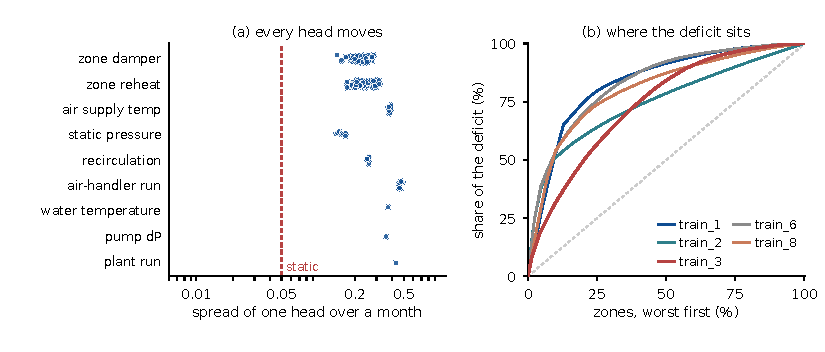
\includegraphics[width=\linewidth]{figures/fig_appendix_behaviour.pdf}
\caption{(a) the spread of each of the 219 heads of the reported checkpoint, median over the months in which that head is active; the dashed line is the threshold below which a head would be called static. (b) the cumulative share of the scored deficit, zones ordered worst first; the diagonal is an even building.}
\label{fig:appendix_behaviour}
\end{figure}

The side of the band differs by building: 87\% and 80\% of the deficit is cold on \texttt{train\_1} and \texttt{train\_8}, 80\% and 78\% hot on \texttt{train\_3} and \texttt{train\_6}, and \texttt{train\_2} is 68\% cold. Figure~\ref{fig:appendix_terms} takes the months one at a time: its three terms, its building, its station, and the side of the band it fails on.

\begin{figure}[h!]
\centering
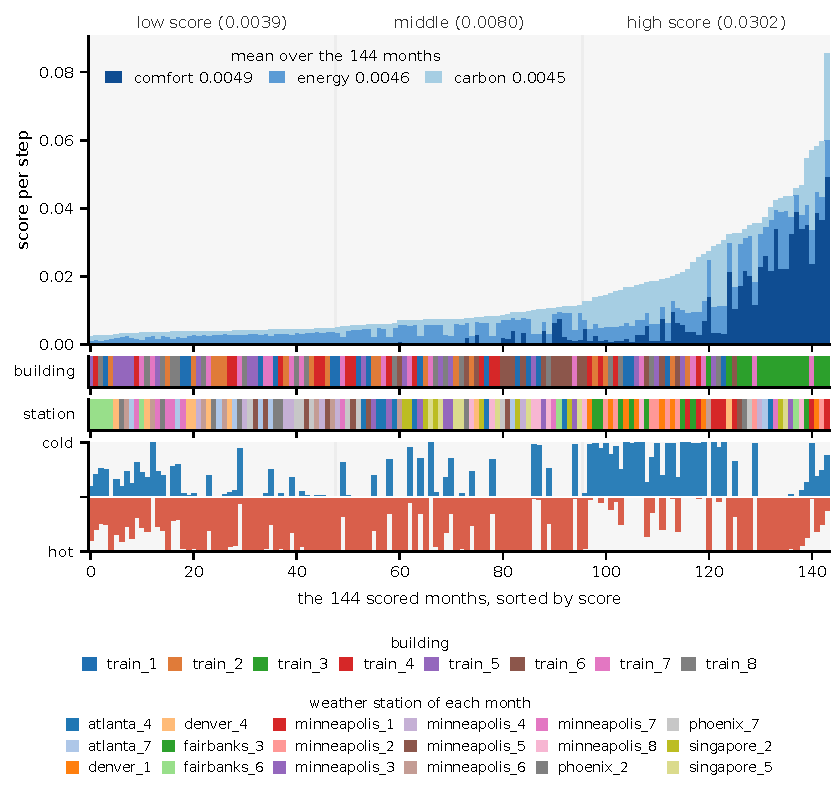
\includegraphics[width=\linewidth]{figures/fig_appendix_terms_labeled.pdf}
\caption{The 144 scored months from both held-out sets, sorted by score and split into thirds. A bar is that month's score split into comfort, energy and carbon; the strips name its building and station; the lower panel says whether the month's out-of-band deviation is cold or hot. \texttt{train\_3} carries 55\% of the top third with 64\% of its bill in comfort, on the hot side, and \texttt{train\_7} is the cold outlier. The other six spend 6 to 34\% on comfort and the rest on energy and carbon.}
\label{fig:appendix_terms}
\end{figure}








\subsection{The Action Follows the Deficit}

The zones in trouble are not the ones receiving less air or heat. On occupied steps the rank correlation between a zone's mean damper position and its mean deficit is positive on all five buildings, from $+0.16$ to $+0.77$: the further out of band a zone sits, the more air it is given.

Reheat looks inconsistent until the sign of the deficit is taken into account, and then it is coherent. On \texttt{train\_1} and \texttt{train\_8}, whose deficit is mostly cold, reheat correlates $+0.49$ and $+0.50$ with the deficit. On \texttt{train\_3} and \texttt{train\_6}, whose deficit is mostly hot, it correlates $-0.51$ and $-0.35$: the hot zones get less reheat. \texttt{train\_2} is the null case at $+0.03$.

The limit of this subsection is the sample. The correlations run across 30 to 85 zones on one pooled set of months, so the intervals are wide and a coefficient near 0.2 is not evidence that the policy cannot aim. What it does show is that the actuators point the right way in the aggregate, so the residual on \texttt{train\_3} is better described as a zone Final cannot hold than as a zone it is not trying to hold.



\subsection{When the Score Accrues}

Table~\ref{tab:app_daypart} gives the score per step in each day-part. The bins here keep weekdays and weekends apart; the hourly curve of Figure~\ref{fig:time}a averages every day of the month, weekends included, so its 06:00 value sits below the weekday morning bin of the table. Day 0 of every episode is an empty Sunday, and Final heats through it: across the five buildings the first 24 hours burn 59, 44, 62, 213 and 294\,kWh of gas, and 57 to 93\% of that falls in the last six hours before comfort starts. That day scores 0.0007 to 0.0020, so the heat is bought at night prices and the bill for it arrives on Monday.

The drift over the 30 days is not uniform. \texttt{train\_3} moves fastest, \texttt{train\_6} and \texttt{train\_2} at about a third and a quarter of that rate ($1.1\times10^{-4}$ and $0.9\times10^{-4}$ per day), and \texttt{train\_1} and \texttt{train\_8} are flat at $5.7\times10^{-5}$ and $3.5\times10^{-6}$. The residual therefore grows on the three largest plants and stays put on the two smallest, which is an early warning for the tail rather than a month that comes apart.

\begin{table}[h!]
\centering
\small
\begin{tabular}{@{}lrrrrr@{}}
\toprule
day-part & PID & SAC & Long & Mid & Final \\
\midrule
weekday night & 0.0037 & 0.0042 & 0.0049 & 0.0064 & 0.0045 \\
weekday morning & 0.1280 & 0.0895 & 0.0633 & 0.0502 & 0.0459 \\
weekday afternoon & 0.1043 & 0.0808 & 0.0585 & 0.0381 & 0.0353 \\
weekday evening & 0.0974 & 0.0826 & 0.0616 & 0.0356 & 0.0326 \\
weekend day & 0.0061 & 0.0002 & 0.0012 & 0.0002 & 0.0001 \\
weekend night & 0.0061 & 0.0006 & 0.0017 & 0.0004 & 0.0003 \\
\bottomrule
\end{tabular}
\vspace{4pt}
\caption{Score per step in each day-part, averaged over the 90 held-out months. A step is five
minutes; the bins are the weekday night (19:00--06:00), morning (06:00--12:00), afternoon
(12:00--16:00) and evening (16:00--19:00), and the weekend day and night.}
\label{tab:app_daypart}
\end{table}

\FloatBarrier




\section{The Off-Policy Baseline}
\label{app:sac}

The SAC arm is CleanRL's \texttt{sac\_continuous\_action.py} with its defaults, run on the same blobs, the same 960 agents, the same 30 scenarios and the same seed as the reported recipe. Table~\ref{tab:app_shared} lists what it shares with our run and what it does not: the contract, the scenario set, the batch, the seed, the actor and the action head are the same; the learner, the critic, the reward normalization and the schedule are not, and the SAC side uses a per-sample entropy target in place of PPO's fixed entropy bonus. The reported arm runs 50{,}135{,}040 steps with the Beta head of Section~\ref{sec:beta_head}, floor 0.5 and cap 12 on $\alpha+\beta$; the same recipe with the Gaussian head is the ablation.

\begin{table}[h!]
\centering
\small
\begin{tabular}{@{}p{0.20\linewidth}p{0.40\linewidth}p{0.32\linewidth}@{}}
\toprule
item & PPO (reported) & SAC \\
\midrule
Simulator, contract & GPU port, 983-vector, 219 heads, $[-1,1]$ & Same \\
Scenarios, agents & 30 shipped, 960 agents, 32 each & Same \\
Seed & 75 & 75 \\
Actor & 80 pooled $\to$ 256; 68/32/16 local; 32-unit zone branch & Same \\
Action distribution & Beta, floor 0.5, cap on $\alpha+\beta$ of 12 & Same \\
Critic & Shared trunk, 90 zone values & One MLP on (observation, action) \\
Gradient passes & 2{,}304 $\times$ 4 per rollout & 2{,}048 $\times$ 2 \\
Reward to learner & Raw, advantages normalized & Per-scenario $z$-score \\
Zone memory & 11 features per zone & None \\
Replay & On-policy & 1{,}048{,}320 transitions \\
Budget & 199{,}895{,}040, annealed to zero & 50{,}135{,}040, no anneal \\
Optimizer & Adam, per-role readouts & Adam \\
Gradient clip & 0.5 & None \\
Truncation & No bootstrap & Terminal at the 8{,}640-step cut \\
\bottomrule
\end{tabular}
\vspace{4pt}
\caption{What the two runs share and what they do not. The comparison controls for the contract, the scenario set, the seed, the actor, the action head and the evaluator; the rows below the actor are what it cannot control for, and the head row is the only difference between the reported arm and its Gaussian ablation (Table~\ref{tab:app_sac_head}).}
\label{tab:app_shared}
\end{table}

The recipe came from a sequence of 50M-step arms on the 30 scenarios, each against a base of four gradient passes and a batch of 256 (Figure~\ref{fig:app_sac_ablation}). The frozen reward normalizer is the worst arm, 0.170 against the base's 0.081; fifteen passes reach 0.071, LayerNorm on that arm does not (0.094), the structured per-zone actor with a batch of 2048 is the best of the sequence (0.026), and adding the zone memory is worse (0.034), so it is left off. The arms form a design sequence rather than isolated single-change comparisons, and no per-change claim is drawn from them. With the Beta head that recipe scores 0.0338 on the 90 held-out months, 27\% below the controller's 0.0461, and 0.0229 on the 54-month extension against 0.0437.

\begin{figure}[h!]
\centering
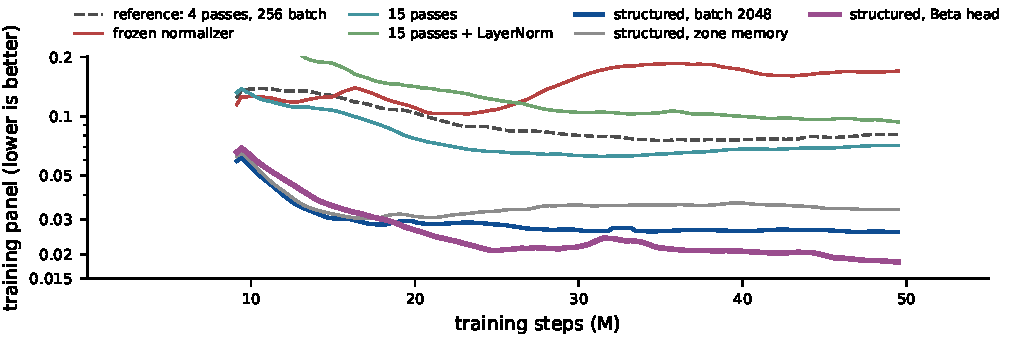
\includegraphics[width=\linewidth]{figures/fig_sac_ablation.pdf}
\caption{The design sequence at 50M steps on the 30 training scenarios, each arm against the base recipe of four gradient passes and a batch of 256. The ordinate is the training panel, the mean episode score over the 30 scenarios, so the curves are the training signal and not the held-out score. The purple curve is the structured recipe with the Beta head, the single change of Table~\ref{tab:app_sac_head}. All arms use one seed, and the curves are smoothed with a five-point mean. Lower is better.}
\label{fig:app_sac_ablation}
\end{figure}

The head is the one member of the set in Table~\ref{tab:app_shared} that can be moved alone. The two 50M runs share the config file, seed 75, the batch of 2{,}048 with two gradient steps per update, the 1{,}048{,}320-transition buffer and the 50{,}135{,}040 steps, and differ only in the head, a tanh-Gaussian against the bounded Beta of Section~\ref{sec:beta_head}. That change lowers the score 26\%, from 0.0457 to 0.0338, and every term: comfort 0.0355 to 0.0262, energy 0.0055 to 0.0048, carbon 0.0047 to 0.0028. Every building improves (Table~\ref{tab:app_sac_head}), and the only one left above the controller is \texttt{train\_3}. The head does not close the gap to the on-policy run, 0.0165 at its full budget and half of 0.0338; the remainder is the rest of Table~\ref{tab:app_shared}, critic and replay and reward normalization and schedule, which this change does not touch. The Beta arm has one budget; more steps under this head are untested. Its public score is 0.0252.

\begin{table}[h!]
\centering
\small
\begin{tabular}{@{}lrr@{}}
\toprule
building & Gaussian & Beta \\
\midrule
\texttt{train\_1} & 0.0241 & 0.0223 \\
\texttt{train\_2} & 0.0262 & 0.0208 \\
\texttt{train\_3} & 0.0901 & 0.0814 \\
\texttt{train\_6} & 0.0644 & 0.0261 \\
\texttt{train\_8} & 0.0237 & 0.0185 \\
\midrule
Months below the controller & 59 of 90 & 81 of 90 \\
\bottomrule
\end{tabular}
\vspace{4pt}
\caption{One recipe, two action heads at 50{,}135{,}040 steps, seed 75, batch 2{,}048 and two gradient steps per update; only the head differs. Each row is the mean over that building's 18 held-out windows on the 90-month set; the totals and the three terms are in the text.}
\label{tab:app_sac_head}
\end{table}

The 200M-budget arm is the same recipe with the Gaussian head, annealed over the longer budget, and it peaks at its first save: 0.0486 at 50M, 0.0567 at 90M, 0.0762 at 120M and 0.0687 at 160M (Figure~\ref{fig:app_sac}), with a public split of 0.0630 at 90M, 0.0775 at 159M and 0.0908 for the completed run, against 0.0640 for the controller. The star in Figure~\ref{fig:app_sac} is the Beta arm at 50M, 0.0338, below the controller where the 200M run's own 50M save, 0.0486, is above it. More budget under the Gaussian head did not buy what the head bought in one change, which is why the 200M arm is the head and budget ablation here, not the reported SAC result.

\begin{figure}[H]
\centering
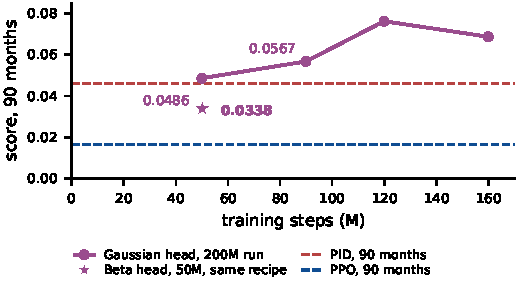
\includegraphics[width=0.55\linewidth]{figures/fig_sac_curve.pdf}
\caption{The 200M-budget run with the Gaussian head, on the 90 held-out months at its four pre-registered saves; it is above the controller at every save and its best save is its first. The dashed lines are the shipped controller (0.0461) and PPO (0.0165). The star is the structured 50M recipe of Table~\ref{tab:app_sac_head} with the Beta head, 0.0338, below the controller at the same budget; its Gaussian counterpart is 0.0457 there, and the curve's own 50M save, 0.0486, is the 200M-anneal recipe. The run was stopped at 168M; the anneal would have reached zero at 200M.}
\label{fig:app_sac}
\end{figure}

\FloatBarrier

\section{Limitations}
\label{app:limits}

Final is one seed. Two seeds at 50M on the four-scenario batch differ by 6\%. The 90-month difference to the controller is far outside that noise, 0.0296 with a 95\% interval of [0.0259, 0.0336] over scenarios (Appendix~F.5) and 89 of 90 months won, but the 11\% gap between the last two saves and the per-building differences are not; the intervals in this paper are over months, not over runs. A second seed at the final scale is the missing replication.

The runs use the benchmark release as shipped. The port matches that release exactly, but a corrected release would change the reference physics or schedules and the recipe would have to be re-validated on it.

The morning bill and the cold months are still high. The weekday morning is the largest bill for every policy, 0.0459 for Final and 0.1280 for the controller per step, and 49\% of the Final-controller gap; the cold windows carry the rest, with Fairbanks at 0.0184, Denver at 0.0181, and the five worst months all in \texttt{train\_3}, whose mean is 0.0443. Final has reduced the morning peak and the cold-month penalty, not removed them, and the residual sits in the first occupied hours of the cold months.

The training set is a design, not a sample: six buildings crossed with five stations, one month per pair. A diversified set, with more buildings, more months per station and a wider generator distribution, should be trained.

The input vector has not been audited for noise. Some of the gateway's 983 values are noisy echoes, some are redundant, and some fields are absent by design, such as per-zone occupancy and weather; a field-level audit that drops and adds one field at a time, scored on the 90 months, would show whether the vector should be reduced or extended.

\end{document}
